\documentclass[12pt,twocolumn,tighten]{aastex62}
%\pdfoutput=1 %for arXiv submission
\usepackage{amsmath,amstext,amssymb}
\usepackage[T1]{fontenc}
\usepackage{apjfonts}
\usepackage[figure,figure*]{hypcap}
\usepackage{graphics,graphicx}
\usepackage{hyperref}
\usepackage{comment}

\renewcommand*{\sectionautorefname}{Section} %for \autoref
\renewcommand*{\subsectionautorefname}{Section} %for \autoref

%% Reintroduced the \received and \accepted commands from AASTeX v5.2.
%% Add "Submitted to " argument.
\received{\today}
\revised{---}
\accepted{---}
\submitjournal{AAS journals.}

\shortauthors{Bouma et al.}
\shorttitle{CDIPS I}

%%%%%%%%%%%%%%%%%%%%%%%%%%%%%%%%%%%%%%%%%%
% BEGIN CUSTOM SHORT-CUT COMMANDS

% BEGIN NUMBERS
\newcommand{\numberpcs}{39\ }  % 2019/06/28 unanimous gold
\newcommand{\numberzaripcs}{10\ }  % 2019/06/28 unanimous gold
\newcommand{\numberclusterpcs}{29\ }  % 2019/06/28 unanimous gold
\newcommand{\sVInumberlcs}{67{,}601\ }  % 2019/06/20 not allnan
\newcommand{\sVIInumberlcs}{91{,}736\ }  % 2019/06/20 not allnan
\newcommand{\numberlcs}{159{,}337\ } % 2019/06/20 sum
\newcommand{\numberclusters}{596\ } % 2019/07/01 paper_plot_all_figures.py
\newcommand{\pctoflcswithage}{77} %  2019/07/02 from hist_logt.png

\newcommand{\stscilink}{\url{archive.stsci.edu/prepds/cdips}}
\newcommand{\stscivetlink}{\url{archive.stsci.edu/prepds/cdips/vetting}}

% END CUSTOM SHORT-CUT COMMANDS
%%%%%%%%%%%%%%%%%%%%%%%%%%%%%%%%%%%%%%%%%%

%%%%%

%\NewPageAfterKeywords

\begin{document}

\title{
  CDIPS. I. Light Curves in Open Clusters from TESS Sectors 6 \& 7
}

\correspondingauthor{L. G. Bouma}
\email{luke@astro.princeton.edu}

\author[0000-0002-0514-5538]{L. G. Bouma}
\affiliation{ Department of Astrophysical Sciences, Princeton
University, 4 Ivy Lane, Princeton, NJ 08540, USA}
%
\author[0000-0001-8732-6166]{J. D. Hartman}
\affiliation{ Department of Astrophysical Sciences, Princeton
University, 4 Ivy Lane, Princeton, NJ 08540, USA}
%
\author[0000-0002-0628-0088]{W. Bhatti}
\affiliation{ Department of Astrophysical Sciences, Princeton
    University, 4 Ivy Lane, Princeton, NJ 08540, USA}
%
\author[0000-0002-4265-047X]{J. N. Winn}
\affiliation{ Department of Astrophysical Sciences, Princeton
University, 4 Ivy Lane, Princeton, NJ 08540, USA}
%
\author[0000-0001-7204-6727]{G. \'A. Bakos}
\affiliation{ Department of Astrophysical Sciences, Princeton
University, 4 Ivy Lane, Princeton, NJ 08540, USA}

\begin{abstract}
  % Context
  The Transiting Exoplanet Survey Satellite (TESS) has begun to
  photometrically monitor almost every star cluster in the solar
  neighborhood.
  % Aims
  Using the TESS images, we have begun a Cluster Difference Imaging
  Photometric Survey (CDIPS), in which we are focusing on stars that
  are candidate cluster members, or else show other indications of
  youth relative to field stars.
  %
  Our aims are to discover giant transiting planets with known
  ages, and also to provide a light curve sample fit for studies in
  stellar astrophysics.
  %
  For this work, we made \numberlcs light curves of candidate young
  stars, across \numberclusters distinct clusters.  Each light curve
  represents between 20 and 25 days of observations of a star brighter
  than $G_{Rp}=16$, sampled at 30 minute cadence.
  % Methods
  We describe the image subtraction and time-series analysis
  techniques we used to create the light curves, which have noise
  properties that agree with theoretical expectations.
  %
  We also comment on the possible utility of the light curve sample for
  studies of stellar rotation evolution, and binary eccentricity
  damping.
  %
  The light curves are available at \stscilink.
\end{abstract}

\keywords{
  planets and satellites: detection  --
  methods: data analysis ---
  techniques: photometric ---
  (Galaxy:) open clusters and associations: general ---
}


%%%%%%%%%%%%%%%%%%%%%%%%%%%%%%%%%%%%%%%%%%



\section{Introduction}
\label{sec:intro}

Each of the $\sim$3000 known star clusters of the Milky Way is a gift
to astrophysics, providing a sample of stars that vary widely in mass
but all have approximately the same age and composition.  Time-series
photometry of clusters has many applications. By measuring rotation
periods over a range of ages, we can study the angular momentum
evolution of stars and improve our ability to determine stellar ages
through gyrochronology \citep[{\it
e.g.},][]{skumanich_time_1972,barnes_color-period_2015,meibom_spin-down_2015,curtis_tess_2019}.
By measuring eccenticities as a function age, we can study the tidal
circularization of binaries
\citep{meibom_robust_2005,milliman_wiyn_2014,price-whelan_binary_2018}.
The detection of eclipsing binaries can also lead to the precise
determination of the absolute dimensions of the stars and stringent
tests of stellar-evolutionary models
\citep{luhman_formation_2012,stassun_review_2014,kraus_mass-radius_2015}.
Finally, transiting exoplanets discovered in clusters can shed light
on the timescales for processes in planet formation, evolution, and
migration
\citep[][]{Fortney_et_al_2007,Mann_K2_33b_2016,David_et_al_2017}, as
well as on the effects of metallicity
\citep[][]{fischer_planet-metallicity_2005,petigura_metallicity_2018}.

The TESS mission \citep{ricker_transiting_2015}, though designed for
other purposes, holds the promise to deliver the most homogeneous and
comprehensive cluster photometric survey in history.  More
quantitatively, the \citet{Kharchenko_et_al_2013} cluster member
database indicates that $\approx 2\times10^5$ open cluster members
brighter than $T=16$ will be observed in the full-frame images over
the first two years of TESS observations.  This count includes the
``most probable'' members within each cluster's radius, which by the
\citet{kharchenko_global_2012} definition requires the independent
kinematic, photometric, and spatial membership probabilities to each
exceed 61\%.  The actual number of stars in clusters is larger, as the
membership catalogs are not yet complete, even at these
relatively bright magnitudes \citep[{\it
e.g.},][]{roser_nine_RSG_2016,cantat-gaudin_gaia_2018,cantat-gaudin_newOCs_2019}.

A major barrier to deriving precise photometry from the TESS images is
the relatively poor angular resolution ($\approx 21''$ per pixel).
Almost all clusters are within 10 degrees of the Galactic plane. The
problems with crowding and complex backgrounds become so severe
that the TESS Candidate Target List deprioritizes
2-minute targets at galactic latitudes less than $\approx
15^\circ$~\citep{stassun_TIC_2018,stassun_TIC8_2019}. This includes
almost all star clusters\footnote{TICv8 updated the cutoff to
$10^\circ$. During the first year of TESS observations, the number
used when selecting 2-minute target stars was $15^\circ$.}.  This decision
was made because
the large pixel size and the high stellar surface density make
aperture photometry unreliable.  However, it means that most
stars in clusters, though capable of yielding a cornucopia of science,
will go unprocessed by the official {\it TESS} data reduction
pipeline.

One way to quantify the blending problem is to determine what fraction of
the total flux in a photometric aperture is contributed by a
particular target star. Aperture photometry is reliable when this
fraction is close to unity.  
Difference imaging \citep{Alard_Lupton_1998,miller_optimal_2008}, in
our group's experience, can be viable down to crowding fractions
of perhaps 1 part in 10.
Based on the
\citet{Kharchenko_et_al_2013} cluster membership data, and the density
of background stars, we calculated that the median dilution fraction of
cluster stars with $T< 16$ is 0.13, for an aperture radius of 2 pixels.
For at least $\sim$$10^5$ cluster stars then, it seems that difference
imaging may be worthwhile.

Difference imaging avoids the primary effects of blending through
forced-aperture photometry.  In this method,
the positions of stars are predicted from an astrometric
solution, and the reference fluxes are determined from a calibrated
catalog magnitude-to-flux relation.  The deviation from the reference
flux is measured on the difference image.  Assuming that only a single
source causes the variability, blended neighbor stars only act to
increase Poisson noise, and do not ``dilute'' transit signals, down to
the angular resolution of the source catalog used to determine the
reference flux.  This is a major benefit of performing image
subtraction in crowded fields.

We have therefore begun to apply difference imaging to the
TESS images, with a focus on any star that could be a member
of a coeval group.  We
are also including some stars that we suspect are young due to
combined photometric and astrometric indicators.
A major motivation for
this effort is to discover giant transiting planets with known ages.
The focus of the present study however is to describe our
methods, and to produce a general-purpose
dataset applicable for studies both in exoplanetary and also
stellar astrophysics.

For the remainder of this work, we adopt the term ``star cluster'', or
simply cluster, to refer to a coeval group of stars.  This includes
the open clusters of yore, as well as the moving groups and stellar
associations that have been discovered since the late
1990s \citep{zuckerman_young_2004}. 

The plan of action is as follows. In \S~\ref{sec:starselection}, we
describe how target stars were selected. \S~\ref{sec:method} presents
the photometric and image processing methods we used to produce light
curves for these stars.  The statistical properties of the \numberlcs
light curves from TESS Sectors 6 and 7 are then summarized
(\S~\ref{subsec:lcstatistics}).  An example of how we might use the
data to identify pulsating stars, eclipsing binaries, and transiting
planets is then given (\S~\ref{subsec:identifying_variability}).
\S~\ref{sec:conclusion} summarizes our findings, and discusses them
with an eye towards the studies we hope this and subsequent rounds of
data processing will enable.


%%%%%%%%%%%%%%%%%%%%%%%%%%%%%%%%%%%%%%%%%%
\section{Method: Star Selection}
\label{sec:starselection}

\begin{figure}[!t]
	\begin{center}
		\leavevmode
		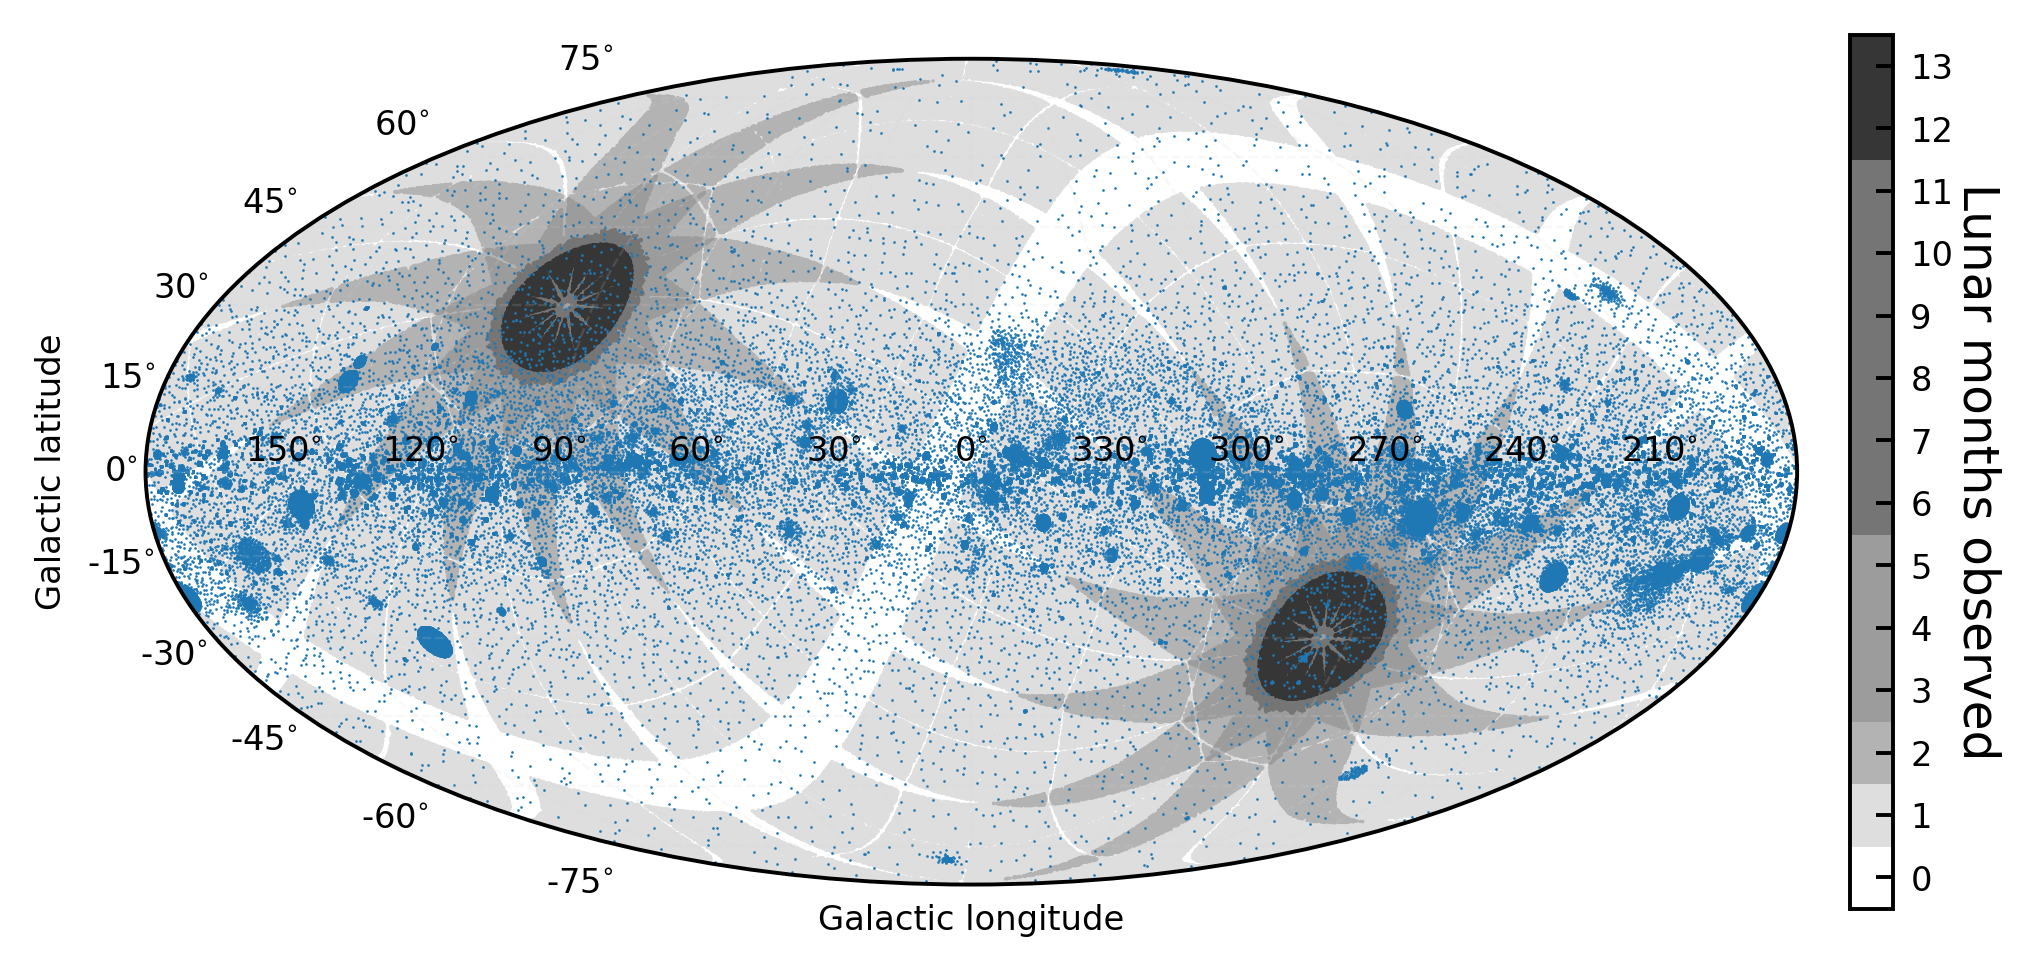
\includegraphics[width=0.48\textwidth]{target_star_positions.png}
		%\gridline{\fig{target_star_cumulative_counts.pdf}{0.41\textwidth}{}}
	\end{center}
	\vspace{-0.5cm}
	\caption{
    Target star positions (blue) and predicted TESS observing
    footprint (gray).  Target stars are either candidate members of
    clusters, or else have other youth indicators (see
    \S~\ref{sec:starselection}).  Most will be observed for one or two
    lunar months over the TESS Prime Mission.
    \label{fig:cdips_targets_positions}
	}
\end{figure}

\begin{figure}[!t]
	\begin{center}
		\leavevmode
		%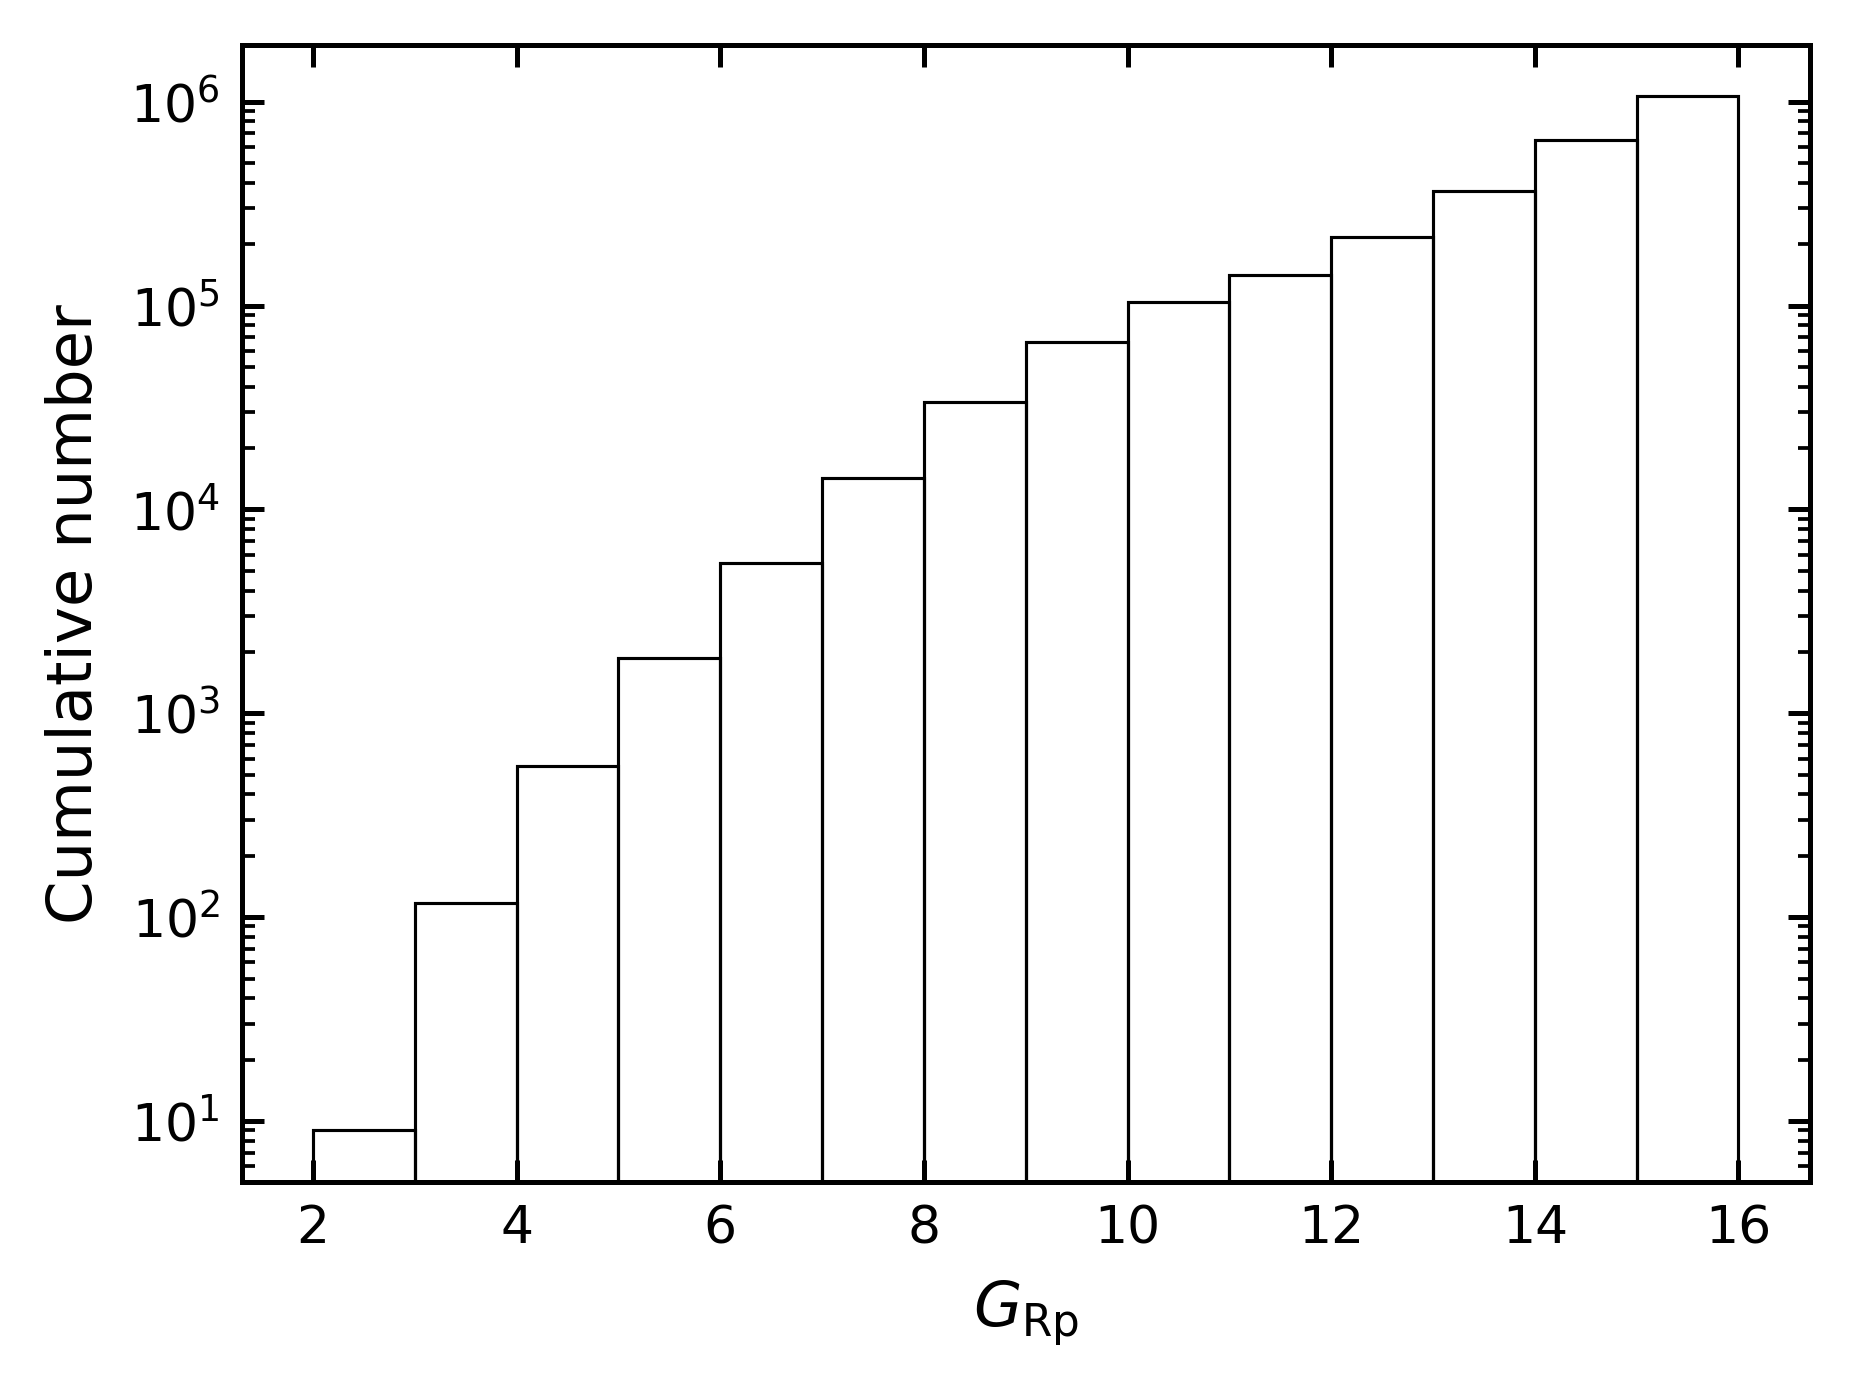
\includegraphics[width=0.45\textwidth]{target_star_cumulative_counts.png}
		\gridline{\fig{target_star_cumulative_counts.pdf}{0.41\textwidth}{}}
		\vspace{-0.8cm}
		\gridline{\fig{target_star_hist_logt.pdf}{0.41\textwidth}{}}
		\vspace{-0.8cm}
		\gridline{\fig{target_star_reference_pie_chart.pdf}{0.41\textwidth}{}}
	\end{center}
	\vspace{-0.8cm}
	\caption{
		Target star statistics.
		{\it Top.} Cumulative counts as a function of Gaia $Rp$-band
		magnitude.  
		{\it Middle.} Histogram of target star ages, for the subset of
		stars with ages matched against \citet{Kharchenko_et_al_2013}.
		{\it Bottom.} Provenance of cluster membership.  Percentages are
		relative to $N_{\rm total}=1061446$ target stars. Symbols
		are as follows.
		D14 is \citet{dias_proper_2014}.
		K13 is \citet{Kharchenko_et_al_2013}.
		CG18 is \citet{cantat-gaudin_gaia_2018}.
		Z18 is \citet{zari_3d_2018}, with upper main sequence and
		pre-main-sequence samples sub-divided.
		``$\geq 2$'' indicates at least two authors reported a star as a
		candidate cluster member.
		%``Other'' refers to sources enumerated in \S~\ref{sec:starselection}.
		\label{fig:cdips_targets}
	}
\end{figure}

\begin{figure*}[!t]
	\gridline{\fig{mwscmatchstats.pdf}{0.75\textwidth}{}}
	\vspace{-0.8cm}
	\gridline{\fig{dias14matchstats.pdf}{0.75\textwidth}{}}
	\vspace{-0.8cm}
	\caption{
		{\it Top.} Quality diagnostics from cross-matching
		\cite{Kharchenko_et_al_2013} cluster members against Gaia-DR2.
		A histogram of the distances between matched stars is on the left; a
		histogram of the difference between the true $G$-band magnitude
		and that predicted from 2MASS photometry is in the middle; a scatter
		plot of the same magnitude difference as a function of $G$-band
		magnitude is on the right.
		{\it Bottom.} Same, but cross-matching \cite{dias_proper_2014}
		cluster members to Gaia-DR2.
	}
	\label{fig:xmatch_info}
\end{figure*}

The main aim of the CDIPS project is to increase the number of cluster
stars for which photometric time-series are available, and thereby
facilitate studies of exoplanetary and stellar processes across
different times and stellar environments.  A key step is
therefore to define a sample of stars that are thought to be young, or
members of clusters, or both.

A homogeneous membership calculation for every known cluster is a
rather large undertaking, and currently falls outside our scope.  So
too is a homogeneous search for young stars across the galaxy.
Instead, we have opted to collect and concatenate appropriate catalogs
from across the literature.  We then use the resulting meta-catalog to
identify our target stars within the TESS images.

The probabilistic criteria for inclusion in our target star list is
necessarily heterogeneous across different catalogs.  However, in our
initial stellar selection we aim for completeness, not accuracy.  If
there has been a claim in the literature that a star should be
considered a cluster member, or a young star, we would like to err on
the side of reporting a light curve for the star.  For stars that are
photometrically interesting, we can then perform post-hoc quality
checks using Gaia-DR2 astrometry and photometry to assess cluster
membership and youth.

\S~\ref{subsec:oc} describes the catalogs we used to identify
candidate members of open clusters.  \S~\ref{subsec:mg} describes the
catalogs we used to identify candidate members of moving groups,
stellar associations, as well as young stars identified through
combined Gaia photometry and astrometry.  \S~\ref{subsec:ocmgsummary}
and Figure~\ref{fig:cdips_targets} describe summary statistics for the
entire sample of about one million target stars.

%FIXME: make table

\subsection{Big catalogs: open clusters}
\label{subsec:oc}

At the time of writing, two relatively large, homogeneous cluster
memberships studies had been performed using {\it Gaia}-DR2: those by
\citet{cantat-gaudin_gaia_2018} and \citet{gaia_hr_2018}.
There were also two large membership studies based on proper motion and 
photometric catalogs that were of interest: the studies of
\citet{Kharchenko_et_al_2013} and \citet{dias_proper_2014}.

\paragraph{{\it Gaia}-derived OC memberships}

\citet{cantat-gaudin_gaia_2018} used the UPMASK unsupervised membership
assignment algorithm \citep{krone-martins_upmask_2014} to identify cluster
members using Gaia-DR2 positions, proper motions, and parallaxes.
They used {\it Gaia} photometry and radial velocities to then verify the
claimed membership properties.  From their Table~2, we collect an initial
401{,}448 cluster members, in 1229 clusters, down to their limiting magnitude
of $G=18$.

\citet{gaia_hr_2018} reported memberships for stars in a smaller, more
select group of well-studied open clusters. From their Table~A1, we
collect 40{,}903 cluster members, in 41 open clusters, mostly within
$500\,{\rm pc}$. While this work also included memberships for
globular clusters, we omitted these from consideration.

Given the unprecedented quality of Gaia-DR2 astrometry, these two
membership sources are our most reliable sources of membership
information.  In our photometric reduction,  our default identifier
for all sources is correspondingly the Gaia-DR2 \texttt{source\_id}.
The TIC identifiers are found through a spatial cross-match after the
light curves have been made, subject to the requirement that the
Gaia-DR2 source identifiers match
\citep{stassun_TIC_2018,stassun_TIC8_2019}.  

% We take this approach
% because Gaia-DR2 is the base-catalog used to project sources from
% celestial coordinates to the imaging plane (\S~\ref{sec:method}).  It
% also has the advantage that for any Gaia-derived cluster memberships,
% we can cross-match directly against source identifiers.



\paragraph{Pre-{\it Gaia} OC memberships}
\citet{Kharchenko_et_al_2013} used proper motions calculated in PPMXL
\citep[][a combination of USNO-B1{.}0 and 2MASS
astrometry]{roeser_ppmxl_2010} and near-infrared photometry from 2MASS
\citep{skrutskie_tmass_2006} to report the existence of 2859 open
clusters and stellar associations (globular clusters were omitted by
excluding any entry of type \texttt{'g'}).  We selected the most
probable cluster members (``$1\sigma$ members'') using the combined
photometric, kinematic, and spatial criteria described by
\citet[][Section~3.3]{kharchenko_global_2012}.  Then, to obtain {\it
Gaia}-DR2 source identifiers for the members, we performed a
crossmatch for {\it Gaia}-DR2 sources within 5 arcseconds of the
listed positions.  To improve the quality of the cross-match, we
additionally used the 2MASS photometry to predict the $G$-band
magnitudes\footnote{See
\url{https://gea.esac.esa.int/archive/documentation/GDR2/Data_processing/chap_cu5pho/sec_cu5pho_calibr/ssec_cu5pho_PhotTransf.html},
online, \texttt{2019-03-29}, or \citet{carrasco_gaia_2016}}, and
required that the measured $G$-magnitude fall within 2 magnitudes of
the predicted $G$-magnitude.  If multiple neighbors matched the
position and magnitude constraints, we took the nearest spatial
neighbor as the match.  From 373{,}226 stars, this yielded a unique
best neighbor for 352{,}332 stars (94.4\% of the sample), and a choice
between two neighbors for 17{,}774 stars. 

%FIXME is this it?
The second (non-{\it Gaia} derived) open cluster membership catalog we
used was the \citet{dias_proper_2014} catalog, which was based on
UCAC4 proper motions acquired by the US Naval Observatory
\citep{zacharias_fourth_2013}.
From their 1805 reported open clusters, we selected sources with
quoted membership probability above 50\%.
To obtain {\it Gaia}-DR2 source identifiers for the members, we
performed a similar crossmatch as before, looking for sources within 5
arcseconds of the listed positions, and within $\pm$2 $G$-band
magnitudes of the prediction.
From 2{,}034{,}269 stars, this yielded a unique
best neighbor for 1{,}828{,}630 stars (89.9\% of the sample), and a choice
between two neighbors for 8.7\% of the remaining sample. 

The distributions of various cross-matching statistics are shown in
Figure~\ref{fig:xmatch_info}.  The distances between matches is
typically below 1 arcsecond.  The Dias catalog shows somewhat stronger
crowding effects at the faint end compared to the Kharchenko catalog,
and likely has a larger number of false matches.
At their faint ends, both catalogs show a tendency for true $G$-band
magnitudes being somewhat larger than predicted $G$-band magnitudes,
presumably due to dust reddening.


\subsection{Smaller catalogs: moving groups and stellar associations}
\label{subsec:mg}

Stars, moving groups and stellar associations are of interest for
similar reasons as stars in open clusters.  Though fewer stars
are known to exist in moving groups, they are of particular interest
because moving groups are less crowded than open clusters, and are
often closer to the Sun.

We obtained Gaia-DR2 identifiers from the results of the following
studies:
\citet{gagne_banyan_XI_2018},
\citet{gagne_banyan_XII_2018},
\citet{gagne_banyan_XIII_2018},
\citet{kraus_tucanahor_2014},
\citet{roser_deep_2011}, % OC, not MG...
\citet{bell_32ori_2017},
\citet{rizzuto_multidimensional_2011},
\citet{oh_comoving_2017}, and
\citet{zari_3d_2018}. The methods applied in these studies
vary from kinematic analyses, to astrometric analyses included
Gaia-DR1 parallaxes, to photometric searches for infrared excesses, to
spectroscopic studies including RVs, H$\alpha$
emission, and Li absorption.

For the Gagn\'e et al{.} catalogs, a large
number of the stars have high proper motions.
However, a number of the stars do not have proper motions quoted.
To perform the cross-match,
we searched the Gaia-DR2 archive for
sources within 10 arcseconds of the listed positions (propagated to the
Gaia-DR2 J2015.5 epoch, if the proper motions were available, otherwise
simply using the listed J2000 positions).
We also imposed a $G<18$ cut on any putative matches. 
We then chose the nearest neighbor by spatial separation.
Of 3012 moving group members collected from the
three combined Gagn\'e et al{.}
catalogs, this procedure yielded 2702 matches.

The \citet{kraus_tucanahor_2014}, \citet{roser_deep_2011}, and
\citet{bell_32ori_2017} studies reported members in Tucana-Horologium,
the Hyades, and 32$\,$Ori respectively.  Applying the same procedure as
for the Gagn\'e catalogs gave 187, 684, and 119 best-neighbors
respectively, compared to 205, 724, and 141 initially reported
members.  Note that \citet{kraus_tucanahor_2014} found that only
$\sim$70\% of their listed members have spectroscopic indicators
consistent with their membership in Tucana-Horologium.

\citet{rizzuto_multidimensional_2011} focused on a single moving
group: the Sco OB2 association. We used their reported Hipparcos
identifiers, and matched against the {\it Gaia} archive's
\texttt{hipparcos2\_best\_neighbour} table, which gave 319
nearest-neighbor stars from 436 candidate members.

Next, \citet{oh_comoving_2017} searched for comoving stars in the
$\approx$2 million stars that overlapped between Tycho-2 and {\it
Gaia}-DR1.  They found many wide binaries, and also identified a large
number of comoving groups.  We chose the 2{,}134 stars that they
reported were in groups with sizes of at least 3 stars.  Using their
{\it Gaia}-DR1 source identifiers, we matched against the {\it Gaia}
archive's \texttt{dr1\_neighbourhood} table, which gave 1{,}881
nearest-neigbor stars in groups of at least three stars
\citep{marrese_gaia_2019}.

Finally, \citet{zari_3d_2018} constructed a sample of young stars
within $500\,{\rm pc}$ using data from Gaia-DR2. Two subsamples were
made: (a) an upper main sequence (MS) sample, with 86{,}102 stars, and
(b) a pre-MS sample, with 43{,}719 stars.  Each was created from a
careful combination of distinct astrometric and photometric cuts.
These stars are the youngest, closest stars, spread across
star-forming complexes in Sco-Cen, Orion, Vela, Taurus, and other
regions of the sky.  Though most of these stars are not directly
identified with moving groups or open clusters, their reported
youth and proximity to star
forming regions justifies their inclusion in our search sample.



\subsection{Summary of target stars}
\label{subsec:ocmgsummary}


After collecting the aforementioned lists, we merged them into a
single table. We queried the \texttt{gaiadr2.gaia\_source} table to
retrieve their photometric $G$, $G_{\rm Rp}$, and $G_{\rm Bp}$
magnitudes, as well as their astrometric measurements $(\alpha,
\delta, \mu_\alpha, \mu_\delta, \pi)$.  Finally, we required that
$G_{\rm Rp} < 16$, which is roughly where the 1-hour photometric
precision of TESS is predicted to reach 1\%
\citep{ricker_transiting_2015}.

All told, this procedure yielded 1{,}061{,}447 unique stars, from 13
distinct membership catalogs.

The relative fractions of stars from each catalog are shown in
Figure~\ref{fig:cdips_targets}.
The largest number of stars come from \citealt{dias_proper_2014}
(44.3\% of stars), \citealt{Kharchenko_et_al_2013} (17.3\%),
\citealt{cantat-gaudin_gaia_2018} (16.7\%), and \citealt{zari_3d_2018}
(11.1\%, of which 7.8\% are OBA stars, and 3.3\% are pre-MS stars).
107{,}647 of the stars, or about 10\%
of the collection, have cluster memberships reported by multiple
authors.  Since the membership probability calculations often use
independent data and methods, agreement between multiple investigators
on a given star's cluster membership is a helpful indication of it
being a bonafide member.
Stars reported in multiple catalogs have all available reference information
concatenated.  

The fraction of target stars from each catalog which are bonafide
cluster members should be understood to be heterogeneous.  For the
\citet{dias_proper_2014} catalog, their membership calculation
included only spatial and kinematic information, and we used a
relatively low probability threshold when including their stars (based
on the criteria \citealt{dias_proper_2014} used for their star
counts).  The \citet{Kharchenko_et_al_2013} catalog combined spatial,
kinematic, and photometric information to derive their membership
probabilities.  We also used a somewhat more restrictive membership
probability cut (again, following the criteria they used for their
star counts), and so this sub-sample is likely less contaminated
with field interlopers.
\citet{cantat-gaudin_gaia_2018} used spatial, kinematic, and
astrometric information from Gaia-DR2. Despite the lack of
photometric information, the quality of the Gaia data suggest that the
field contamination rate will be lowest for the
\citet{cantat-gaudin_gaia_2018} sample.


To assign unique cluster names, we adopted the name matched against
\citet{Kharchenko_et_al_2013} whenever possible.
Appendix~\ref{appendix:uniquenames} describes  how this was done in detail.
For moving groups not identified in \citet{Kharchenko_et_al_2013}, we used
the constellation-based naming convention from
\citet{gagne_banyan_XI_2018}.  Otherwise, we used the name reported by
the original catalog claiming membership.  This process reduced 16,425
name permutations down to 3,216 unique cluster names.  Though we have
made every effort to avoid duplicates, a small number may remain, so we
advise inspection of the \texttt{cluster} column
as well as the references given in the
\texttt{reference} column rather than using the
\texttt{unique\_cluster\_name} column to analyze individual objects
of interest.  Nonetheless, 87.7\% of the $\sim$million unique target
stars are matched to clusters within \citet{Kharchenko_et_al_2013},
and 88.8\% are assigned a cluster name.  The remainder are mostly the
young stars from \citet{zari_3d_2018}.
Ages and their uncertainties are then merged against the 
parameters reported by \citet{Kharchenko_et_al_2013}.

The resulting CDIPS target star list is given in Table~N.
The cumulative distribution of target star brightnesses, as well as a
histogram of the ages, is shown in Figure~\ref{fig:cdips_targets}.
Relative to field stars, our target star sample is young, with a
typical age of 100$\,$Myr.






%%%%%%%%%%%%%%%%%%%%%%%%%%%%%%%%%%%%%%%%%%
\section{Method: Photometry}
\label{sec:method}

\begin{figure}[!t]
	\begin{center}
		\leavevmode
		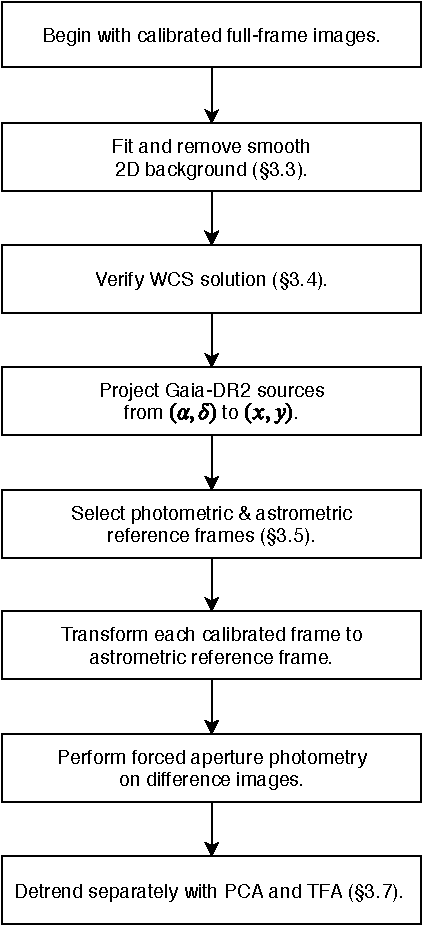
\includegraphics[width=0.3\textwidth]{pipelineoverview.pdf}
	\end{center}
	\vspace{-0.2cm}
	\caption{
    Conceptual overview of photometric reduction pipeline.
    Details are given in \S~\ref{sec:method}.
    %TODO: add latex section numbers!
    %TODO: do FORCED aperture photomery on differenced images
    %TODO: improve text generally
	\label{fig:pipeline}
	}
\end{figure}

\begin{figure*}[!t]
    \begin{center}
        \leavevmode
        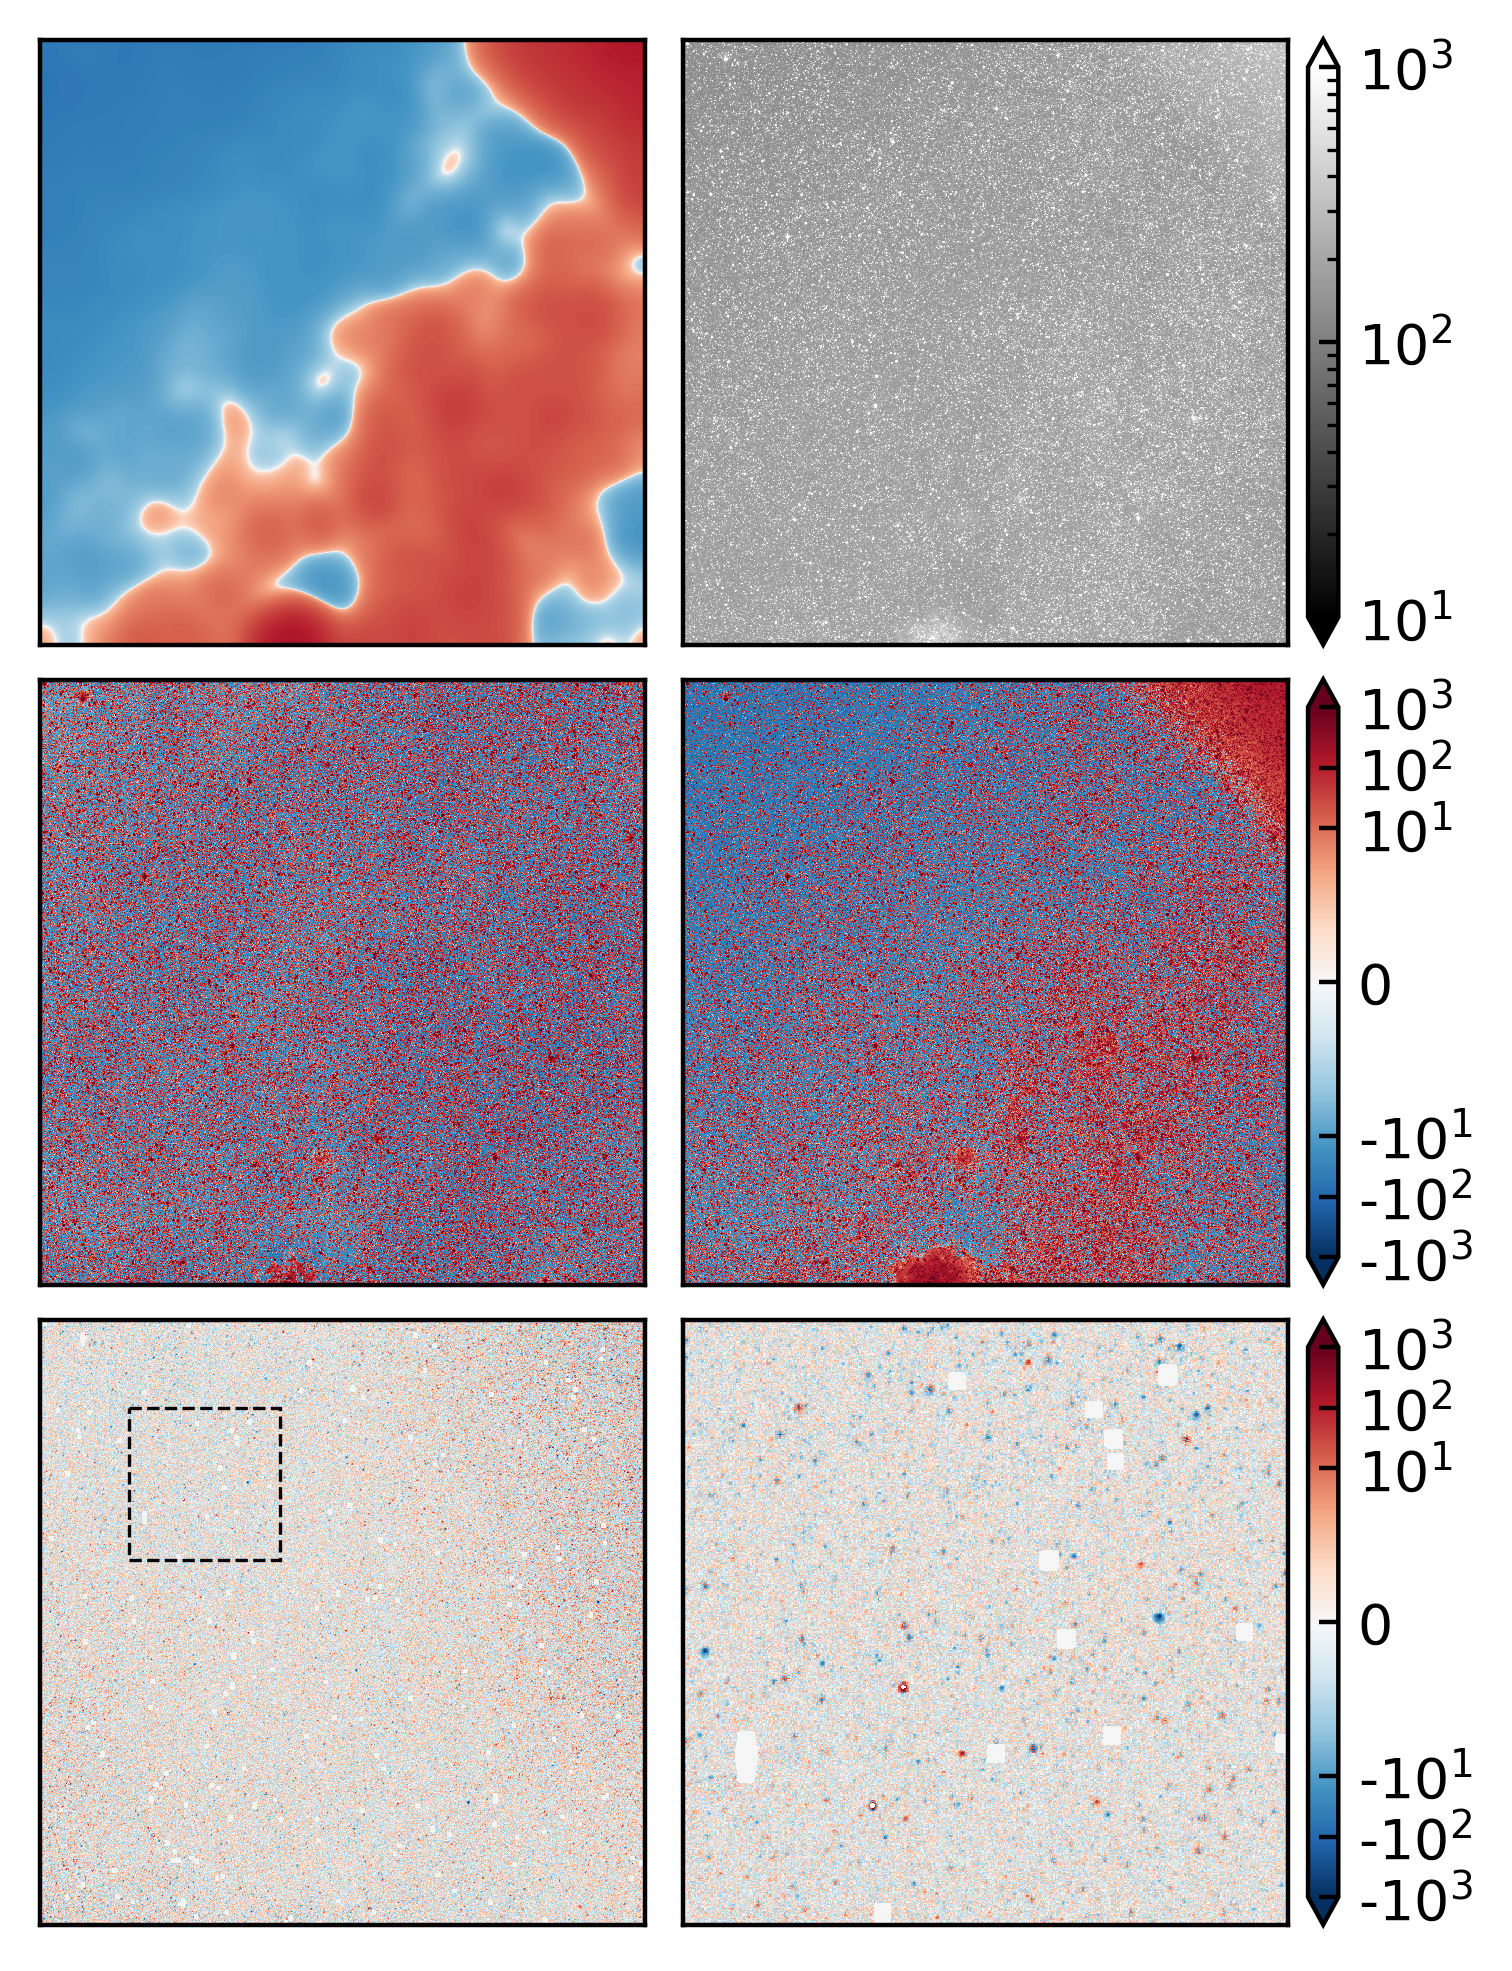
\includegraphics[width=0.95\textwidth]{stages_of_image_processing_good.png}
    \end{center}
    \vspace{-0.6cm}
    \caption{
        Stages of image processing for an image taken during the middle
        of an orbit.
        {\it Top right}. Calibrated image.
        {\it Top left}. Smooth background estimate.
        {\it Middle right}. Calibrated image minus its median pixel value.
        {\it Middle left}. Calibrated image minus smooth background.
        {\it Bottom left}. Registered difference image.
        {\it Bottom right}. Zoom of difference image.
        Each image is $(2048\times2048)$ pixels, except for the bottom-right 
        image, which is $(500\times500)$.
        All images except the top-right have the same color map.
        The sector, camera, and CCD are (6, 1, 2).
        \label{fig:stages_good}
    }
\end{figure*}

\begin{figure*}[!t]
    \begin{center}
        \leavevmode
        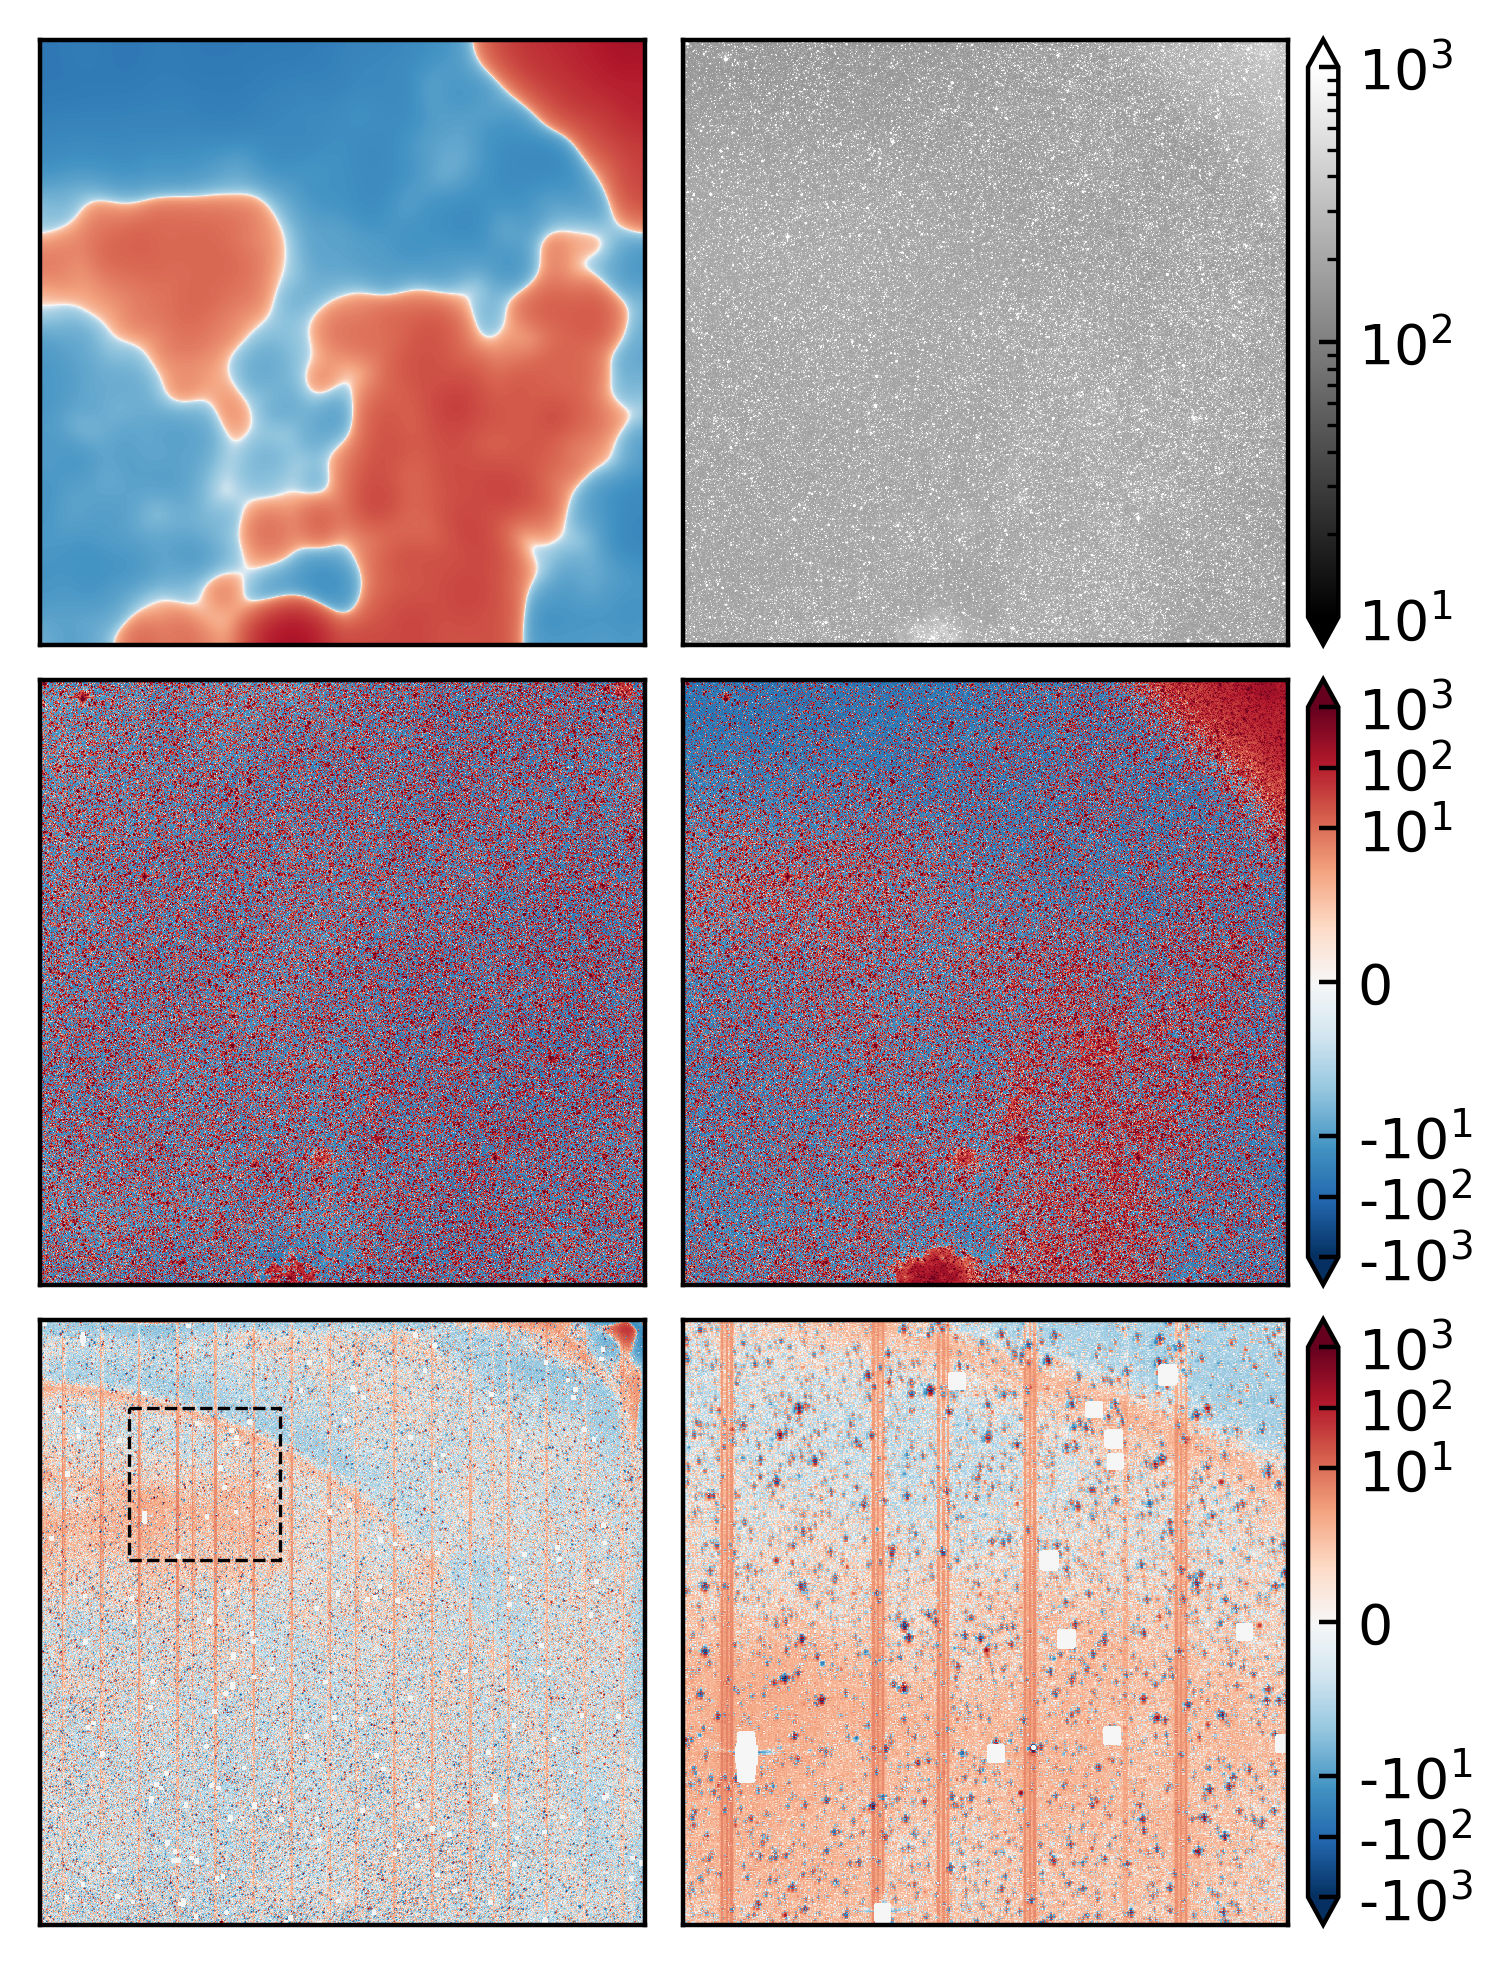
\includegraphics[width=0.95\textwidth]{stages_of_image_processing_bad.png}
    \end{center}
    \vspace{-0.6cm}
    \caption{
        Same sector, camera and CCD as Figure~\ref{fig:stages_good}, but for an image taken during
        perigee passage, when scattered light from the Earth is
        prominent.
        A number of systematic artifacts are present,
        including vertical ``straps'' and small-scale structure in scattered light
        patches.
        The quality of astrometric registration in the difference image is also
        worse, leading to larger residuals in the lower-right panel.
        \label{fig:stages_bad}
    }
\end{figure*}

\subsection{Overview}

To reduce the TESS images to light curves, we adopted a
difference imaging approach.  The overall method is in the spirit of the
reduction pipelines developed by \citet{Pal_2009},
\citet{huang_high-precision_2015}, \citet{soares-furtado_image_2017}
and \citet{oelkers_precision_2018}; a conceptual overview is given in
Figure~\ref{fig:pipeline}.  Most sub-modules of our pipeline have been
developed over the past decade to process HAT data \citep[{\it
e.g.},][]{bakos_hat_review_2018}.  The specific high-level framework
used for this reduction was adapted from a pipeline called
\texttt{pipe-trex}, under development primarily for the HATPI project
(\url{hatpi.org}).  The code is available
online\footnote{\url{github.com/waqasbhatti/pipe-trex}, commit
\texttt{cd9f9bb}.}.

We begin our processing with the calibrated full frame images produced
by the Science Processing Operations Center at NASA Ames
(\S~\ref{subsec:observations}).  We then perform a collection of
preparatory steps, including source extraction of bright stars,
astrometric verification, and coarse simple aperture photometry of
bright stars (\S~\ref{subsec:preparation}).  Using the information
collected from these initial steps, we select an astrometric reference
frame to which we transform all of the calibrated images.  We
construct a photometric reference by stacking a subset of these
transformed frames, after having convolved the frames to have
identical stellar profiles. Finally, we subtract each target frame
from the photometric reference (\S~\ref{subsec:imagesubtraction}).  We
perform aperture photometry on the subtracted images using positions
projected onto the frame from the Gaia-DR2 source catalog.  We detrend
the resulting light curves (\S~\ref{subsec:lcdetrending}).  The
resulting white noise and red noise properties of the light curves,
and a few interesting cases of variability, are discussed in
\S~\ref{sec:results}.


\subsection{Observations}
\label{subsec:observations}

% How did TESS observe?
% What processing steps happened in order to get the calibrated frames?
% Why did we choose to start with them?

The TESS spacecraft began science operations on July 25, 2018.  To
keep its cameras pointed opposite the Sun, the spacecraft advances by
$\approx$$28$ degrees east in ecliptic longitude every lunar month.
Data acquired throughout each ``sector'' are downlinked at spacecraft
perigee through the Deep Space Network.  Descriptions of the
spacecraft's design and operations are given by
\citet{ricker_transiting_2015} and the instrument handbook
\citep{vanderspek_2018}.

For us, the main data product of interest is the calibrated full frame
image (FFI).  Each TESS camera is read out every 2 seconds.  To
produce a manageable telemetric load, the resulting pixel values are
averaged by the onboard computer into 30 minute exposures. An on-board
cosmic ray mitigation algorithm is applied \citep[][\S
5.1]{vanderspek_2018}. Once transmitted to the ground, the raw images
are calibrated by the Science Processing Operations Center (SPOC).  The
calibration process includes an overscan, bias, and dark current
correction, and also divides out a flat field.  Details are discussed
by \citet{clarke_kepler_2017}, and the resulting science data products
are described by \citet{tess_data_product_description_2018}.

We perform our processing using the calibrated images, their
corresponding uncertainty images, and the associated headers.  The
spacecraft has four cameras, and each camera has four CCDs.  In the
following analysis, all image-level operations are thus performed on
the images for each CCD, so that at any instant of time there are 16
independent images that require analysis.

While we performed numerous initial tests on the first sectors of
data, by geometric coincidence Sectors 1--5 were pointed away from the
galactic plane.  Consequently, less than 2\% of the CDIPS target star
sample was observed in the first five TESS sectors.  Though a few
interesting clusters are present in these observations ({\it e.g.},
Blanco~1, NGC~2516, NGC~1901), for the present work we opted to focus
on sectors in which there were more stars of interest for our intended
science.  These begin in Sector 6 (2018-12-12, spacecraft orbit \#19).
For this run of processing, they conclude at the end of Sector 7
(2019-02-01, spacecraft orbit \#22).
Sectors 6 and 7 cover galactic longitudes from roughly 200$^\circ$ to 280$^\circ$, 
with fair coverage within $\pm 20^\circ$ of the galactic plane
(Figure~\ref{fig:cdips_targets_positions}).


\subsection{Image preparation \& background removal}
\label{subsec:preparation}

Before we can perform any kind of photometry, a few janitorial tasks
are required.
First, we convert the multi-extension calibrated FITS image from MAST
into a single-extension FITS image, and trim to remove virtual rows
and columns using the \texttt{SCIROWS}, \texttt{SCIROWE},
\texttt{SCCSA}, and \texttt{SCCED} header values.

In order to preemptively address the background variations present in
some frames due to scattered light from the Earth and Moon
\citep[see][\S 7.3.1--7.3.4]{vanderspek_2018}, we then estimate and
subtract the large-scale background.  We do this by temporarily
masking out pixels more than $2\sigma$ from the image median, and then
pass a $48\times48$ median box filter over each pixel in the image,
with reflective boundary conditions.  The resulting background
estimate has low-amplitude structure over spatial scales of a few
pixels, so we then blur it with a gaussian kernel to produce a smooth
background estimate for each image.  These steps also remove a
low-level vignetting present in the corners of many images, which
remains even after flat-fielding \citep[see][\S
7.3.5]{vanderspek_2018}.  
The results are shown in the upper four panels of Figures~\ref{fig:stages_good}
and~\ref{fig:stages_bad}.
Features with spatial scales smaller than $\approx$48 pixels remain, 
but large scale scattered light patches are removed.

% We found this background subtraction step to be particularly important
% in our subsequent difference imaging analysis. In its absense, the
% scattered light artifacts could introduce erroneous residuals into the
% kernel solution used to match reference and target images.  Including
% this step mitigated such effects, and helped produce clean
% subtractions.  Even after subtraction, a small fraction of frames also
% show sharp features (caustics) below our median box filter's size
% scale.  Such features may affect flux measurements at specific times
% in a small subset of light curves.

After subtracting the background, we mask out saturated pixels using a
fixed saturation level of $8\times10^4\,{\rm ADU}$. This value was
chosen based on the onset of bleeding charge trails in the images, and
is slightly greater than the saturation level of $2\times10^5$
electrons, or about $4\times10^4\,{\rm ADU}$, quoted by
\citet{vanderspek_2018}. 
We correspondingly do not analyze stars brighter than $T\approx 6.5$.
As described by \citet{Pal_2009}, the pixel masks are metadata to the
image, and are only applied to the pixel values during the specific
image processing steps in which they are necessary ({\it e.g.},
convolution). We also extend the masks beyond purely saturated pixels
to ``bloomed'' pixels horizontally and vertically adjacent to the
saturated pixels (see Figure~6 of \citealt{Pal_2009}).

Finally, for frames with the \texttt{DQUALITY} bit-flag corresponding
to the ``momentum dumps'' and ``coarse pointing modes'' described by
\citet{vanderspek_2018}, we omit the entire frame.  This removes on
average a few frames per sector, out of about one thousand. Through
visual inspection, we see that the stars on these frames are extremely
smeared, and are unlikely to produce useful science data.  In
addition, we use the sector-specific data release notes\footnote{\url{
  archive.stsci.edu/tess/tess_drn.html}} to identify further times
with anomalous spacecraft performance, which we omit from
consideration.  For Sectors 6 and 7, this included three days at the
beginning of Sector 6 dedicated to acquiring pixel response function
data, and no additional gaps in Sector 7.
%For Sectors 1 through 5, these
%include coarse pointing windows from orbits 10, 13, 14, and an
%instrumetal anomaly window in orbit 15.
% For Sectors 6 through 8, these include three days at the beginning of
% Sector 6 dedicated to acquiring pixel response function data, and also
% about three days during Sector 8 lost to an instrument anomaly.

\subsection{Metadata collection \& WCS verification}
\label{subsec:metadatacollection}

\begin{figure}[!t]
	\gridline{\fig{astromresidual_hist.pdf}{0.5\textwidth}{}}
	\vspace{-0.8cm}
	\gridline{\fig{astromresidual_quiver.pdf}{0.5\textwidth}{}}
  %\vspace{-0.8cm}
	%\gridline{\fig{astromresidual_apertures.pdf}{0.5\textwidth}{}}
	\vspace{-0.8cm}
    \caption{
		{\it Top.} Histogram of astrometric residual. The $x$-axis shows 
		the distance between the measured centroid positions of stars, 
		compared to the predicted positions from the WCS solution.
		{\it Bottom.} Vector plot of astrometric residual. Each arrow is 
		the vector from the measured to the projected star position. 
		Directions are correct, but lengths are 50 times their true size for 
		visualization purposes.
    The systematic error in the top-right corner is a typical
    problem generic to wide-field astrometry.
    The frame chosen for this plot is the photometric reference frame used 
    for Sector 6, Camera 1, CCD 1; we automatically 
    impose cutoffs on the median and $90^{\rm th}$ percentile of the 
    astrometric residual in order to ensure similar levels of astrometric 
    precision are maintained throughout the reduction.
	}
	\label{fig:astromresid}
\end{figure}

Having prepared the images, we perform some initial analysis steps to
produce metadata needed during image subtraction.  

First, we perform source extraction on the
thousand or so brightest, non-saturated stars in each image.  
This is done using a \texttt{fitsh} tool, \texttt{fistar}.
We derive centroid positions for the stars, and
simultaneously
fit elongated gaussians to their profiles, yielding the shape
parameters $(s,d,k)$, where the flux $f$ as a function of position
$(x,y)$ in the CCD image plane is assumed to take the form
\begin{align}
  f(x,y) &= B + A \exp \{ -0.5 \times [
    s(\Delta x^2 + \Delta y^2) + \\
    \nonumber
    &d(\Delta x^2 - \Delta y^2) +
    k(2\Delta x \Delta y)
  ]  \},
\end{align}
for $(x_0,y_0)$ the central coordinates of the star,
$\Delta x = x-x_0$, $\Delta y = y - y_0$, $B$ the background
level, and $A$ an arbitrary
flux-scaling constant.
For a nearly circular shape profile, the sharpness $s$ is related to
the FWHM as ${\rm FWHM} \approx 2.35\sqrt{s}$ \citep[{\it
e.g.},][]{Pal_2009}.  These shape parameters are later used when
selecting an astrometric reference frame
(\S~\ref{subsec:imagesubtraction}).  
In agreement with what is obvious upon visual inspection, this 
fitting process shows that stars closer to the
center of each camera's field are round, while
stars near the field edges are more triangular.

For the astrometric solution, we use the World Coordinate System (WCS)
and fourth-order Simple Imaging Polynomial (SIP) coefficients
derived by SPOC and included in the FFI headers
\citep[][Sec.~8]{pence_fits_2010}.  We explored the possibility of
using \texttt{astrometry.net} \citep{lang_2010} to derive our own
astrometric solutions for each frame, but found that the astrometric
residual (the mean separation between projected and measured
positions) was consistently a factor of 1.5-2 times higher in our WCS
solutions than in those given by SPOC.  This was perhaps because
we did not develop a robust
algorithm to select non-blended stars of intermediate brightness before
measuring their positions.
Nonetheless, we did find that extending the astrometric correction
to sixth order (compared to the fourth-order polynomial coefficients
in the SPOC solution) did not improve the quality of the fit. 

With the resulting WCS information, we then project a source catalog
onto each frame. 
We use the
projected positions of the sources to center the apertures in our
photometry,
rather than attempting to detect the positions.  Such
``forced-aperture photometry'' is preferable to source
extraction in the crowded fields that are central to this work.  The
Gaia-DR2 epoch is J2015.5, so even the fastest-moving stars with
proper motions of $\sim$$1\,{\rm arcsecond}\,{\rm yr}^{-1}$ are still
well within one pixel of their predicted positions in the TESS images.
The projection from catalog sky-coordinate positions to pixel
coordinates is performed using an analog of the \texttt{wcs-rd2xy}
program that performs the standard matrix algebra \citep{lang_2010}.
The source catalog look-up is performed using
\texttt{gaia2read}\footnote{\url{github.com/samuelyeewl/gaia2read}}
\citep{kim_2018_gaia2read}.

For the source catalog itself, we initially planned to photometer all Gaia-DR2
sources in each field down to a cutoff of $G_{Rp} < 16$.  However,
for the galactic plane fields this produced an excessively
large number of sources (millions of stars per
$12^\circ\times12^\circ$ CCD).  We therefore limited our source
catalog for each frame to be
a combination of the CDIPS target stars ($G_{Rp} < 16$), and
all Gaia-DR2 sources down to $G_{Rp} < 13$.  
The latter set of stars are used for image processing and
light curve detrending.

The residual between the measured and projected stellar centroid
positions is displayed for one photometric reference frame in
Figure~\ref{fig:astromresid}.
The construction of this frame will be described shortly, however
a few salient points can first be made.
First, the typical median precision of the WCS solution is a bit below
0.1 pixels, and its $90^{\rm th}$ percentile is typically less than
0.3 pixels\footnote{In fact, in our reduction we automatically impose
that the median residual and 90th percentile remain below 0.2 and 0.4
pixels, respectively.}.
%The distribution has a outlier tail of saturated stars which were
%masked, and thus do not have measureable centroid positions.
The errors are typically largest in the corners of the field of view,
where the non-linearity of the focal plane is most significant, and
the corrections required by the SIP coefficients are largest.
%The final sub-panel of Figure~\ref{fig:astrometricresidual} is a
%sanity check on the location of the projected positions, and also
%gives some context for our chosen aperture radii of 1, 1.5, and 2.25
%pixels.

Finally, to collect the metadata needed
to select photometric reference frames,
we perform
aperture photometry on the
bright stars.
This task is
performed by using \texttt{fiphot} to
sum the counts inside 
circular apertures centered on the projected stellar positions.
The pixel weights are equal to the fraction of the pixel
that falls within the aperture.  They are unity for pixels
entirely within the aperture, and fractional along the aperture
boundary. % (see \citealt{Pal_2009} Fig 17). 
The background levels are measured in annuli around each aperture
center. 
%The raw flux of the object after background removal is then
%(\citealt{Pal_2009} Eq 65)
%\begin{equation}
%  f = \sum_{x,y} w_{x,y} (I_{x,y} - B) = f_{\rm total} - B r_0^2.
%  \label{eq:simple_aperture_phot}
%\end{equation}
The resulting measurements, for instance of the background level of
each aperture, and the number of stars with ``good'' photometry,
can then be used to assess the photometric quality of each frame.


\subsection{Image subtraction}
\label{subsec:imagesubtraction}

\subsubsection{History of image subtraction method}

The core operation of ``classical'' image subtraction attempts to
match a photometric reference $R$ and a target image $I$ by computing
and applying a convolution kernel.  For ground-based data, this
``match'' typically corrects for differences in seeing or transparency
between the reference and target; for space-based data, the match
might correct for spacecraft jitter, or thermal and corresponding
point-spread function (PSF) variations.  The kernel, once applied to
the high signal-to noise reference, produces a model image, $M_{xy}$,
\begin{equation}
    M_{xy} = (R \otimes K)_{xy} + B_{xy},
    \label{eq:imagemodel}
\end{equation}
where $B_{xy}$ is a component of the model image that allows for
background variations, and $\otimes$ denotes convolution.  Since we
modeled the background separately (\S~\ref{subsec:preparation}), we
set $B_{xy}=0$.  The convolution kernel $K$ is typically decomposed
onto a basis, $K = \sum_i c_i K_i$, and the coefficients are found by
minimizing
\begin{equation}
    \chi^2 = \sum_{xy} \left( \frac{I_{xy} - M_{xy}}{\sigma_{xy}} \right)^2,
    \label{eq:chisq_conv}
\end{equation}
where $\sigma_{xy}$ is the uncertainty in the target image pixel
values.  Photometry is then performed on the difference image
$D_{xy}$, where $D_{xy} = I_{xy} - M_{xy}$.  For the present
reduction, the uncertainty in each target image pixel was taken to be
a constant.	

The general procedure described above was first proposed by
\citet{Alard_Lupton_1998}.  It was reviewed and clarified by
\citet{miller_optimal_2008}.  The choice of how to decompose the
kernel was further explored by \citet{bramich_new_2008}, who showed
that using a linear combination of delta functions (also called
a ``discrete kernel'') had advantages
compared to a basis of gaussians.  We perform the convolution using
\texttt{ficonv}, and opt for the implementation of Bramich's method
(see \citealt{Pal_2009} \S~2.8).  The lower panels of
Figure~\ref{fig:stages_good} show the procedure working well, and
producing a ``clean'' difference image.  Figure~\ref{fig:stages_bad}
shows what happens for an image taken when scattered light from the
Earth causes the model image to be a poor fit to the target
image.


\subsubsection{Astrometric registration}

To make the above high-level picture work, we need to select
two ``reference frames'':
(1) the astrometric reference; and (2) the photometric reference.

To choose the astrometric reference, we search for frames with
large, round stars (big $s$, small $d$ and $k$ values).  We also
require that the frame have minimal background noise, as measured in
annuli around the bright stars selected in
\S~\ref{subsec:preparation}.  Finally, the astrometric reference
needs to have, relative to the other frames being considered, a large
number of detected sources (though the variance between frames was rather 
small).  We sort the frames
using these metrics, and then select the astrometric reference from
successive intersections of each sorted list.

We then compute and apply a spatial transformation of each calibrated
frame to match the astrometric reference frame.  This
transformation~--~a combination of rotation, dilation, and
translation~--~typically moves stars by less than a pixel, since the
TESS spacecraft pointing is quite stable.  We calculate the transformation
using the measured source positions found in
~\S~\ref{subsec:metadatacollection}, and the symmetric triangle
point-matching scheme described by \citet[][~\S~2.5.2]{Pal_2009}.
This step is achieved using the \texttt{fitsh} tools \texttt{grmatch} and
\texttt{grtrans}.  To help ensure the precision of the transformation,
we require the ``unitarity'' $\Lambda$
\citep[][~Eq.~54]{Pal_2009}, which characterizes the degree of
distortion in the transformation matrix, to be below 0.01.  To
mitigate possible photometric errors incurred during this step, we
also use the flux-conserving interpolation scheme described by
\citet{Pal_2009}, which is necessary because polynomial interpolation
schemes do not conserve stellar flux. 

\subsubsection{Photometric reference frame construction \& reference flux measurement}

The second required reference frame is the photometric reference,
which is used both to calculate the convolution kernel, and to obtain
a reference flux for each star.  To make it, we first choose 50 images
with low background measurements (measured for each frame from the
annuli around bright stars), and only consider frames with a
relatively large number of detected bright objects.  We then convolve
these candidate photometric reference frames to the frame with the
lowest background measurement, and construct the photometric
reference as the median image across the 50 frame stack. 

Measuring the reference flux for each star is a non-trivial
operation.  First, we perform forced simple aperture photometry on the
photometric reference frame to measure the flux for each source.  The
local background is estimated in annuli, with neighboring stars masked
out during the background measurement.  If we were to stop
here, {\it it would be a bad mistake}.  The reference fluxes for faint
stars would be overestimated, due to crowding.  The relative amplitude
of photometric signals for faint stars would correspondingly be biased
small, which would hinder exoplanet detection, among other
applications.

To avoid this problem, after performing simple aperture photometry on
the reference frame, we fitted a line between the catalog $T$-band
magnitude of each star, and its measured flux.  The $T$-band magnitude
was calculated according to Equation~1 of \citet{stassun_TIC8_2019}.
We then use the known catalog magnitude to predict the expected
reference flux for each star.  This minimizes crowding down to Gaia's
resolution limit of $\approx$1$''$, rather than the TESS limit of
$\approx$20$''$.

The final instrumental flux
values $f$ we report are given by \citep[][Equation~83]{Pal_2009} 
\begin{align}
f &=  f_{\rm reference} + f_{\rm subtracted} \\
&=
g \left(T_{\rm cat} \right)
+
\frac{1}{|| K ||_1^2} \sum_{x,y} D_{x,y} (w \otimes K)_{x,y}.
\label{eq:ism_flux_measurement}
\end{align}
The function $g$ takes as input the target star's catalog magnitude
$T_{\rm cat}$, and returns the reference flux.  Its coefficients have
been fit per the procedure just discussed, independently for each
aperture.  The difference image $D$ is equal to $I -  R\otimes K$,
where as in Equation~\ref{eq:imagemodel}, $I$ is the target image
transformed to the astrometric reference, $R$ is the photometric
reference, and $K$ is the convolution kernel.  The weights $w$ from
the circular aperture mask are included in the convolution.  The norm
$|| K ||_1$ is defined by \citet{Pal_2009}~Equation~81.

\subsection{Choice of convolution kernel}

To solve for the coefficients to the convolution kernel, a
few further assumptions are necessary.  The procedure implemented in
\texttt{ficonv} is to subdivide the image, and within each grid
element find the brightest non-saturated star. These isolated
``stamp'' stars are then used to solve for the coefficients of the
kernel, by minimizing Equation~\ref{eq:chisq_conv} over the sum of all
stamps.  For the kernel basis, we use a linear combination of
delta functions with a flux scaling term
(\citealt{soares-furtado_image_2017} Section 3.3.1 gives the
equations).  In this model, spatial variations of the PSF across the
image are captured by weighting each basis component with spatial
polynomials up to a cut-off order.

%NOTE : this is kind of incomprehensible
%CHECK: does the polynomial weighting actually do what you want it to do?

This kernel model has three free parameters: (1) the box-size; 
(2) the maximum order of the polynomial weighting the delta
function terms; (3) the maximum order of the polynomial weighting the
flux scaling.  We performed a grid-search to tune these parameters, in
which our ``loss functions'' were the measured RMS as a function
of magnitude, and the recovered SNR of transits from the catalog
of known TOIs (TESS Objects of Interest; N.~Guerrero, in prep).

In the first dimension, we varied the kernel size between a box of
$3\times3$ pixels and $11\times11$ pixels.  Increasing the kernel
box-size from a $3\times3$ box to a $7\times7$ box led to about a 50\%
lower light curve RMS for bright stars, and no difference for faint
stars.  The largest kernels, of $(11\times11)$ pixels, returned
slightly lower signal-to-noise for recovered transits than kernels
of intermediate size.  We settled on a kernel box-size of $(7\times7)$
pixels, which is $\approx$2 times larger than the typical TESS FWHM
at field center. 

In the other two dimensions, we varied the spatial polynomial orders
weighting the kernel's individual pixels between first and fifth
order.  We did the same for the polynomial weights of the ``identity''
pixel.  Varying the polynomial orders between 1 and 4 did not produce
large differences.  The fifth order polynomials retrieved transits
with $\approx10\%$ worse SNR compared to lower order polynomials.  We
therefore adopted a second order polynomial weight in both terms.

Averaging over all TOIs present in the camera we used for these
experiments, we found that different choices of kernel parameters
produced variations of $\lesssim 12\%$ in the retrieved transit SNR.  
For computational expediency, we therefore chose a single $(7\times
7)$ kernel with second-order spatial polynomial weights in the basis
functions for the remainder of our reduction.

However, we caution that within these fine-tuning experiments, we
found that transit signals near the noise floor could fall under the
noise floor for different cases of tuned parameters.  In the longer
term, developing an image-subtraction method that marginalizes over
uncertainties of how to chose ``optimal'' kernels would be desirable.
Pixel-level image subtraction methods that omit these parameters
entirely are similarly worth exploring \citep{wang_pixel-level_2017}.

With a kernel selected, and the convolution and subtraction performed,
we calculate the instrumental fluxes for each frame per
Equation~\ref{eq:ism_flux_measurement}.  We did this with three
different aperture sizes: for this work, circles of radii 1 pixel, 1.5
pixels, and 2.25 pixels.  These sizes were chosen to roughly span the
range of optimal aperture sizes for stars in our sample, as calcuated
from the pre-flight \citet{Sullivan_et_al_2015} noise model.  Finally,
to convert from a list of flux measurements for each source on a frame
to a list of flux values at any given time, we used the
\texttt{fitsh} transposition tool \texttt{grcollect}.

\subsection{Light curve detrending}
\label{subsec:lcdetrending}

\begin{figure*}[!t]
	\gridline{
    \fig{detrended_light_curves_sec6cam1ccd4.pdf}{0.5\textwidth}{}
    \fig{detrended_light_curves_sec7cam3ccd2.pdf}{0.5\textwidth}{}
  }
	\vspace{-0.5cm}
	\caption{
    Twenty randomly selected light curves drawn from the same sector,
    camera, and CCD, for CDIPS target stars with $T$-band magnitudes
    between 13 and 14.  For each star, we show the raw light curve
    (top), PCA-detrended light curve (middle), and TFA-detrended light
    curve (bottom).  The sector, camera, and CCD numbers are 6, 1, 4
    (left) and 7, 3, 2 (right).  A number of systematic trends are
    shared across raw light curves ({\it e.g.}, the periodic $\sim$3 day
    ``chopping'' seen in the left plot).  In the PCA light curves,
    stellar rotation signals are usually preserved, but not always ({\it
    e.g.}, left panel, seventh from the top).  TFA filters out almost
    all long-term trends, or else heavily distorts them ({\it e.g.},
    right panel, fourth from the bottom)
	\label{fig:lc_systematics_dtr}
	}
\end{figure*}

\begin{figure}[!t]
	\begin{center}
		\leavevmode
		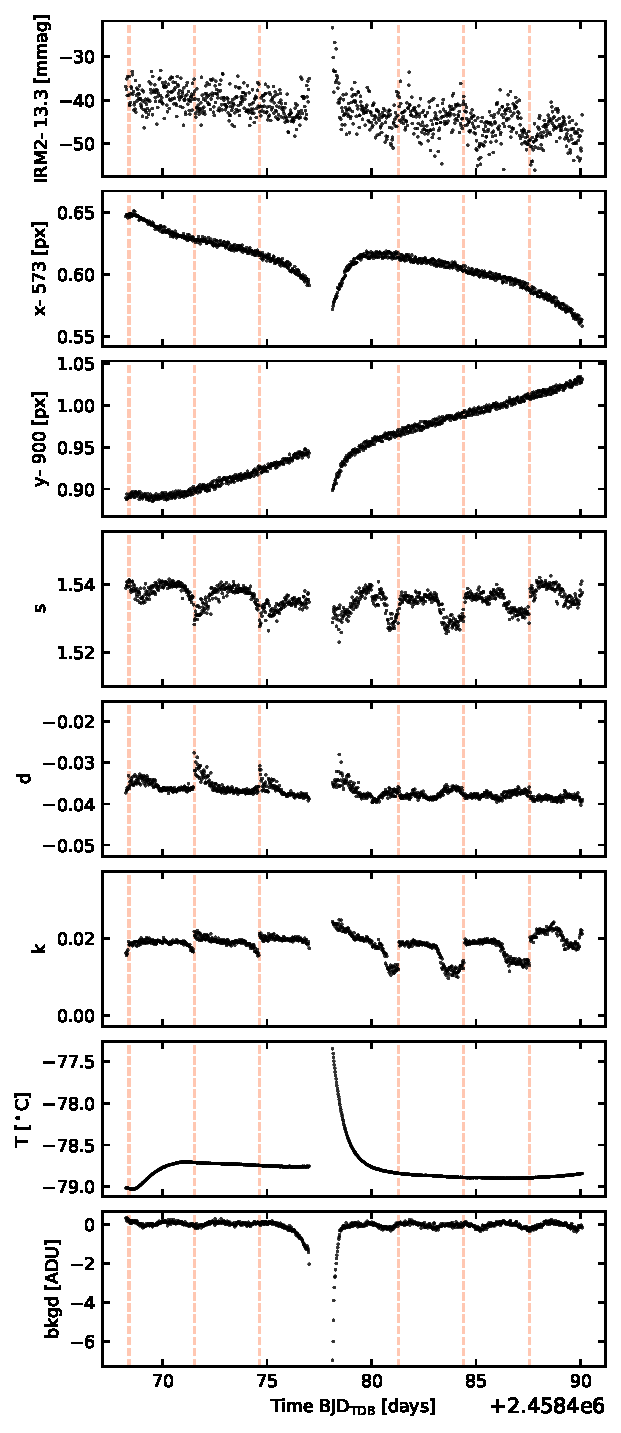
\includegraphics[width=0.44\textwidth]{external_parameters_vs_time_sec6cam1ccd1.pdf}
	\end{center}
	\vspace{-0.5cm}
	\caption{
    The variability in flux is sometimes correlated with variability
    in ``external'' parameters, shown here for a representative star
    over two orbits.  {\it Top}: Instrumental raw magnitude (with a
    particular aperture size), as a function of time.  Continuing in
    order are $x$ and $y$ centroid positions as a functions of time,
    the $(s,d,k)$ PSF shape parameters, the CCD temperature,  and the
    measured background value.  Differential aberration affect the
    centroid position over the span of each orbit.  Momentum dumps are
    marked with vertical dashed lines, and affect the measured shapes
    of stars.
		\label{fig:external_parameter_timeseries}
	}
\end{figure}

The preceding steps produce light curves that include both
instrumental systematics as well as astrophysical variability.
Figure~\ref{fig:lc_systematics_dtr} shows twenty stars of comparable
brightness randomly selected from two CCDs.  Stars that are far apart
on the same CCD often share similar changes in flux.  In other words,
the instrumental systematics seem to dominate.  This problem is
generic to most wide-field photometric datasets, including the WASP,
Kepler, and HAT surveys
\cite{Pollacco_2006,borucki_kepler_2010,bakos_hat_review_2018}.  To
remove the systematic variability, we adopted two different
approaches: {\it (i)} the trend-filtering algorithm (TFA,
\citealt{kovacs_trend_2005}), and {\it (ii)} a principal component
analysis (PCA).

However, a number of other approaches to the problem were possible. To
encourage future improvements, we describe the possibility of
decorrelating against external parameters
(\S~\ref{subsubsec:external}), and also different available approaches
to ensemble detrending (\S~\ref{subsubsec:ensemble}), before
explaining our adopted implementation.


\subsubsection{Decorrelating against external parameters}
\label{subsubsec:external}

Often, ensemble trends of stellar magnitude with CCD position,
sub-pixel position, catalog magnitude, and color are present in
datasets.  One detrending step that can be valuable is to fit and
subtract a linear combination of these trends as they appear across
many light curves \citep[{\it e.g.},][\S~5.5]{zhang_precision_2016}.

A separate step for each light curve can then be to fit out linear
correlations of stellar magnitude with ``external parameters'' (EPD,
\citealt[][]{bakos_2010,huang_high-precision_2015}).  For ground-based
data these parameters might include zenith angle, or changing PSF
shape.  For TESS data, they might include CCD temperature, or the
angles of the Moon and Earth relative to each camera's boresight.
They might also include the standard deviation of the spacecraft
quartnerion time-series \citep{vanderburg_hr858_2019}.  Some example
``external'' parameters that we include with our light curves are
shown as functions of time in
Figure~\ref{fig:external_parameter_timeseries}.

We explored the possibility of fitting linear models of flux as
functions of {\it e.g.,} temperature, shape parameters, and centroid
positions to each light curve.  We also briefly explored non-linear
model fitting using $N$-dimensional B-splines to fit the flux,
centroid positions, and temperatures simultaneously
\citep{dierckx_curve_1996}.  The linear models typically underfit the
light curves, particularly during the large shifts that happen as the
spacecraft nears perigee.  The non-linear models showed some promise,
but often seemed to overfit stellar variability signals.  Given these
complications, for the time being we omitted the step of
``detrending'' as a function of external parameters. To enable further
exploration of the issue, we included all the necessary vectors of
{\it e.g.}, centroid positions, temperatures, and shape parameters in
our reported light curves.

\subsubsection{Ensemble detrending}
\label{subsubsec:ensemble}

The parameters that capture systematic trends are often poorly known.
In such cases, an effective model of the systematics comes from
constructing a set of vectors that empirically captures trends common
to many stars.  Each target light curve is then assumed to be a linear
combination of the trend vectors.

The well-known algorithms, TFA, Sys-Rem, PDC-MAP, and ARC2, all take
slightly different approaches to constructing this set of basis
vectors, as well as to solving for the weights to assign each linear
component
\citep{kovacs_trend_2005,tamuz_correcting_2005,smith_pdc_2012,aigrain_robust_2017}.
TFA selects individual ``template stars'' as basis vectors, and
equally weights each template when solving for the coefficients via
linear least squares.  PDC-MAP computes ``co-trending basis vectors''
(CBVs) by applying singular value decomposition to the light curves
that show the strongest mutual correlation.  It solves for the
coefficients through a two-step procedure.  The first step is to
calculate the coefficients through linear least squares.  The
least-squares coefficients are then used to construct a prior over
plausible coefficient values, which is subsequently used to recompute
the maximum likelihood coefficients for each star.  This latter step
reduces overfitting for stars with variability not present in the set
of CBVs.

We opted to use two different detrending approaches, each aimed
at a different use case.  For transit-search related science,
we used TFA, as implemented in \texttt{VARTOOLS}
\citep{kovacs_trend_2005,Hartman_Bakos_2016}.  For stellar
astrophysics related work, we used a simple variant of PCA, as
implemented in \texttt{scikit-learn} \citep{sklearn_2011}.  For
self-consistency, we describe each method and its implementation in
the following paragraphs.

\paragraph{TFA detrending}

The idea of TFA is as follows.  Suppose we have $M$ ``template
stars'', which are a subsample of stars that represent all types of
systematics across the dataset.  Each template star has a light curve
with $N$ data points.  Denote the template time-series $X_j(i)$, where
$j={1,\ldots,M}$ and $i={1,\ldots,N}$ is the time index.  We then want
to find periodic signals in a target time-series $Y(i)$.  This is done
by defining a filter function
\begin{equation}
  F(i) = \sum_{j=1}^{M} c_j X_j(i),
\end{equation}
for which the coefficients $c_j$ are found by minimizing
\begin{equation}
  \mathcal{D} = \sum_{i=1}^{N} \left[ Y(i) - A(i) - F(i) \right]^2.
  \label{eq:tfa_to_minimize}
\end{equation}
When trying to find periodic signals, $A(i)$ represents our prior
knowledge of the light curve's shape.  This prior is simply that stars
on average maintain a constant brightness:
\begin{equation}
  A(i) = \langle Y \rangle = \frac{1}{N} \sum_{i=1}^{N} Y(i) = {\rm const.}
\end{equation}
If a signal is eventually found, for instance using the box-least
squares method \citep{kovacs_box-fitting_2002}, this detrending
process must then be repeated while accounting for our updated
knowledge about the light curve's shape.

Some implementation notes follow.  We selected template stars in two
stages.  In the first stage, we fitted a parabola in the RMS-magnitude
plane, and discarded stars more than $2\sigma$ away from the
prediction of the fit.  We also required that these initial candidate
stars have intermediate brightness ($8.5 > T > 13$), and have a
relatively large number of time-series data points.  We then performed
an initial iteration of TFA, on only the candidate template stars.  We
inspected the resulting detrended light curves for residual structure
by computing a Lomb-Scargle periodogram.  If the maximum-power peak
had a false alarm probability below 0.1\%, we excluded the star from
the list of candidate template stars, on the basis of its presumed
periodic variability.  We then randomly selected at most 200 template
stars from the remaining non-variable candidates.  The choice of
number of template stars was discussed by \citet{kovacs_trend_2005},
and is another free parameter in the broad problem of light curve
production.  This choice is analogous to the issue of how many
cotrending basis vectors to choose in PDC-MAP or ARC2
\citep{aigrain_robust_2017}.  While the number of template stars can
be optimized by constructing and minimizing a BIC-like quantity, a
little overfitting is acceptable for our pupose of finding planetary
transits.  For other applications, {\it e.g.,} stellar rotation period
searches, it is almost certainly preferable to adopt a less forceful
detrending approach.

\paragraph{PCA detrending}

To remove the largest systematic trends with minimal overfitting of
{\it e.g.}, stellar rotation signals, we adopted a simple variant of
PCA (see {\it e.g.}, \citealt{ivezic_statistics_2014} for a review).
A similar approach was taken by \citet{feinstein_eleanor_2019} in
\texttt{eleanor}.  We derived the principal components for each CCD
using the 200 template stars previously selected for TFA.  We then
modelled each target light curve as a linear combination of a subset
of these principal components, with weights determined by linear least
squares.

To determine the ``optimal'' number of principal components to use, we
performed a cross-validation analysis on the template stars using the
components derived both from PCA, as well as a separate factor
analysis.  As is typically the case when the noise variance is
different for each ``feature'' (each point in time), we found that
$k$-folding cross-validation using PCA failed to recover a plausible
number of components\footnote{See for example
\url{https://scikit-learn.org/stable/auto_examples/decomposition/plot_pca_vs_fa_model_selection.html}}.
However, the factor analysis typically maximized the cross-validation
score with anywhere from $10$ to $15$ components, which agreed with a
visual analysis of the number of PCA components past which overfitting
began.  We therefore used the maximum cross-validation score from
thefactor analysis as the number of principal components to use in
each light curve.  This number is documented in the \texttt{FITS}
header of each light curve.

% In \S~\ref{sec:flux_vs_external_parameters}, we describe the
% ``external parameter'' dependence visible in our reduction of
% the TESS data.
% Ordinary linear model-fitting, as well as an initial attempts
% at non-linear model fitting, are poor descriptions of the data.  
% In a similar vein ``magnitude-fitting'' is minimally justified, given
% how the TESS magnitudes correlate against these external parameters.
% We go on to show (\S~\ref{sec:tfa_is_good_enough}) that a plausible
% detrending approach for the purpose of transit discovery is to simply
% decorrelate against other nearby stars with standard TFA.
% 

% \subsubsection{Flux versus external parameters}
% \label{sec:flux_vs_external_parameters}
% 
% 
% % \begin{figure*}[t]
% %     \begin{center}
% % 		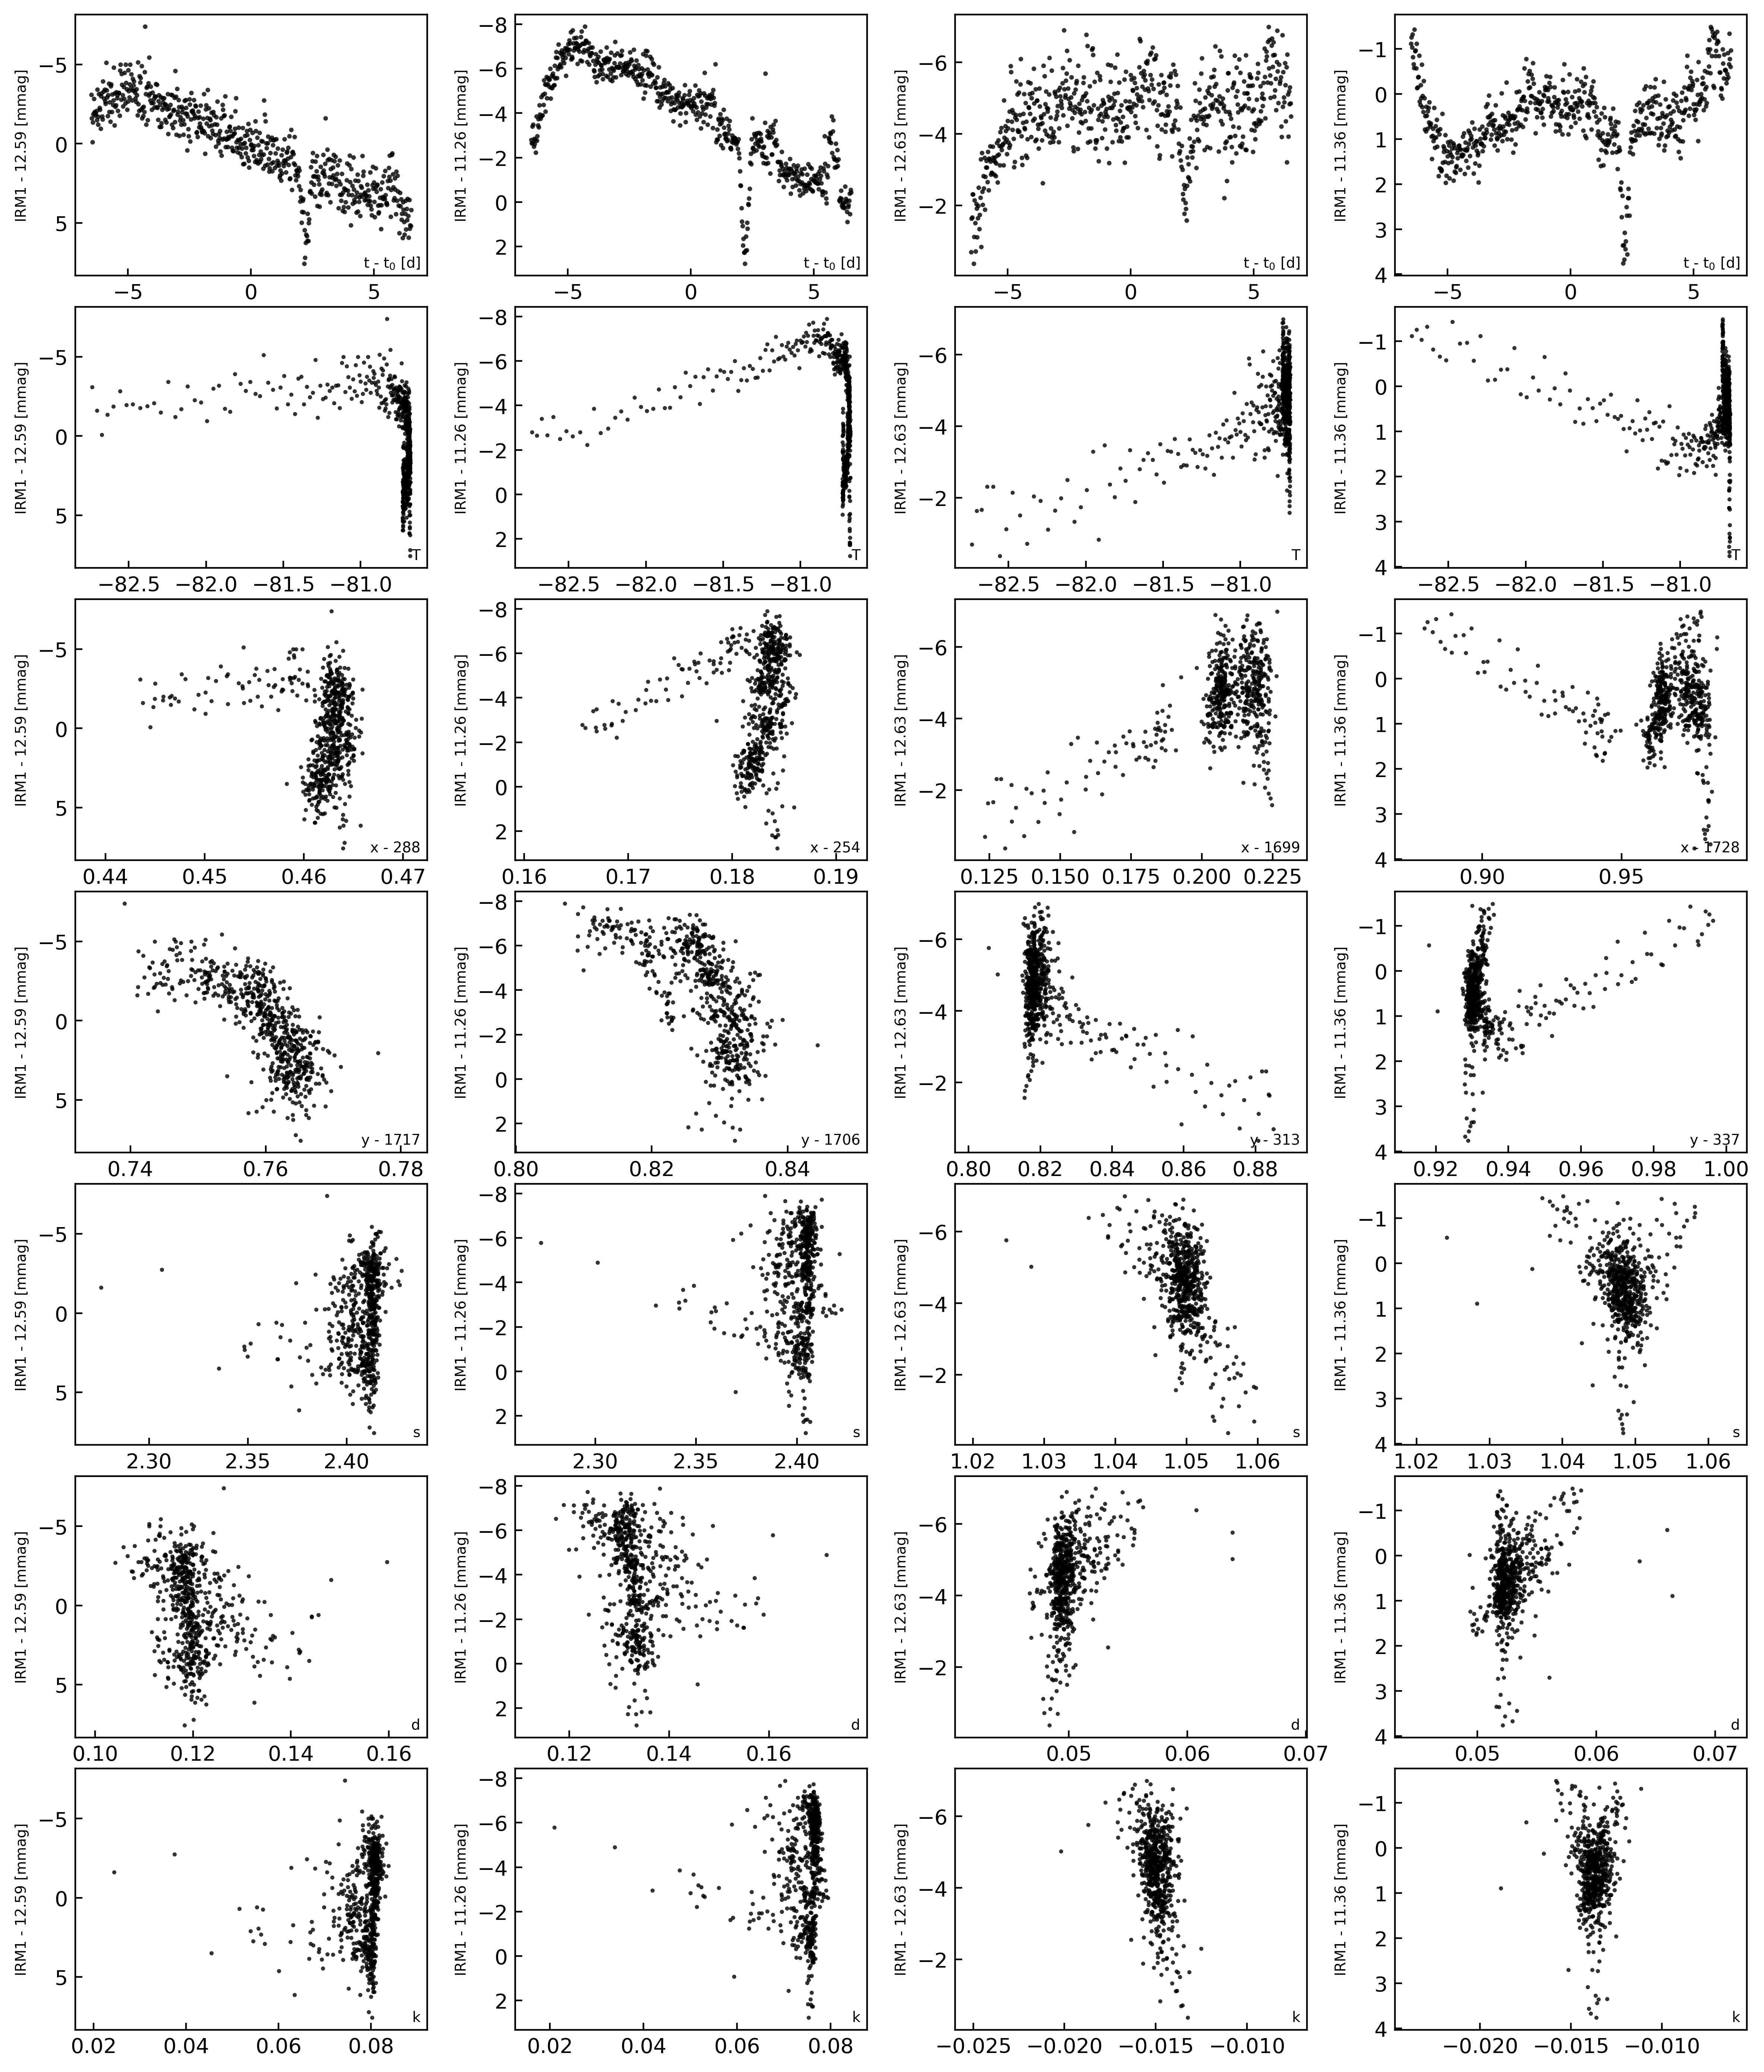
\includegraphics[height=0.9\textheight]{mag_vs_epdparams.png}
% %     \end{center}
% %     \vspace{-0.5cm}
% %     \caption{
% %       {\bf Flux as a function of ``external parameters'' for four
% %       representative stars.} The left two columns are stars at the
% %       corner of a camera's field; the right two columns are from the
% %       centers.
% %       Each row shows a different parameter along the $x$-axis, given
% %       in text at the bottom right of each subplot.
% %       ``Hooks'' are common features in flux as a function of
% %       temperature and centroid position.
% %       \S~\ref{sec:flux_vs_external_parameters} gives a verbose
% %       description.
% %      \label{fig:flux_vs_external_parameters}
% %     }
% % \end{figure*}
% 
% The traditional approach to EPD is to fit and
% subtract a model for the magnitudes $m$ of the form
% \begin{equation}
%   m = {\rm const.} + \sum_i c_i \theta_i,
%   \label{eq:classical_EPD}
% \end{equation}
% where $\vec{\theta}$ is a vector of parameters such as the shape
% parameters $(s,d,k)$, their products $(s^2, s\cdot d, d^2, \ldots)$,
% the temperature $T$ of the instrument or environment\footnote{ We used
% the temperature from the on-chip aluminum-copper sensor measurements
% included in the engineering
% data: \url{archive.stsci.edu/missions/tess/engineering/}.  },
% the centroid positions $(x,y)$, the fractional part of the
% centroid positions $(\{x\},\{y\})$, and any other parameters that are
% expected\footnote{ The fractional centroid positions might matter
% because intra-pixel quantum efficiency variations could affect the
% measured stellar brightness.  The varying temperature $T$ of the CCD
% electronics might matter.  } to correlate strongly with the observed
% flux.  The coefficients $c_i$ are calculated through linear
% least-squares, and subtracted to produce ``EPD'' light curves.
% 
% The premise of this model is that the correlations between the
% magnitudes and the external parameters are linear.  For ground-based
% CCD data (e.g., HATNet, HATS, and Nikon DSLRs), \citet{bakos_2010} and
% \citet{zhang_precision_2016} have verified that this model is a
% good description to the data.
% To discern whether such a model extends to the TESS data, we examined
% scatter plots of each parameter, as a function of all the other
% parameters.  We also examined plots of each parameter as a function of
% time.  A few prominent trends were present.
% 
% \begin{enumerate}
% 
% \item {\it Flux vs.\ time}. Most of the light curves we examined showed a secular
%     drift with amplitude $0.01\,{\rm mag}$ over the timescale of each
%     orbit.  Sharper trends (``hooks'') at the beginning of each orbit
%     seemed to be less prominent for stars at the corners of the fields
%     than stars at the center.  The periodicity incurred by the
%     2.5$\,{\rm day}$ momentum dumps was also noticeable in more of the
%     light curves at the center of the field than at the corners.
% 
% \item {\it Flux vs.\ centroid positions}. The flux as a function of
%   centroid position often showed non-linear ``hooks''
%     %(see Figure \ref{fig:flux_vs_external_parameters}).
%     Most of the data points from a given orbit reside at a given
%     level, but about 10\% are in a tail. This was seen in light curves
%     all across the TESS field of view.
% 
% \item {\it Flux vs.\ temperature} exhibited similar hooks, with most of
%   the flux values residing at a particular level, and perhaps 10\%
%     following a non-linear path (often resembling the Nike ``swoosh'')
%     away from the bulk of points.
% 
% \item {\it Flux vs.\ shape parameters}.  For light curves in the corner
%   of the field of view, similar hooks are present in flux {\it vs.}
%     $(s,d,k)$, though the hooks are less sharp.  In the center of the
%     field of view, gaussian ellipses are a better description of the
%     flux {\it vs.} the shape parameters.
%     
% \end{enumerate}
% 
% Considering the timeseries of parameters other than flux 
% (Figure~\ref{fig:external_parameter_timeseries}):
% 
% \begin{enumerate}
% 
% \item {\it Centroid positions vs\ time}.  The main variability in the
%   centroid positions as a function of time is a secular drift, that is
%     reset every orbit.  The 2.5 day momentum wheel dump is
%     superimposed on this secular drift, and has smaller amplitude than
%     the drift.
% 
% \item {\it Temperature vs.\ time}.  The main variability in temperature
%   {\it vs.} time is a secular drift of the same timescale as that for
%     the centroid positions timeseries.
% 
% \item {\it Shape parameters vs.\ time}.  The main variability in the
%   shape parameters as a function of time is the 2.5 day momentum wheel
%     dump periodicity, with hooks before each momentum dump.
% 
% \item {\it Background value vs.\ time}.  The background is typically stable, 
% except when scattered light from the Earth or Moon enters the frame (visible 
% towards the end of each orbit in 
% Figure~\ref{fig:external_parameter_timeseries}).
% 
% \end{enumerate}
% 
% Given the characteristics of the variability, a linear model of the
% form given in Equation~\ref{eq:classical_EPD} is not applicable.  To
% fit out the correlations between flux and parameters which most
% commonly exhibited ``hooks'', we explored fitting a parametric open
% curve (an $N$-dimensional B-spline, \citealt{dierckx_curve_1996}) to
% the flux, centroid positions, and temperatures simultaneously.  We
% selected the number of knots through brute-force, by calculating
% $\chi^2$ for the model fit over a grid of possible knots, and
% minimizing the Bayesian Information Criterion.  Though this approach
% showed some initial promise, even with ``optimal'' knot-selection (in
% the BIC sense) it introduced undesirable residuals in the light curves,
% and also distorted transits.
% One thought that we did not try but may explore in future work
% is to use the decorrelate against the scatter of the quartnerion 
% time-series \citep{vanderburg_hr858_2019}.
% 
% Given these complications, for the time being we omit the step of
% ``detrending'' as a function of external parameters. To
% enable further exploration of the issue, we include all the necessary
% vectors of {\it e.g.}, centroid positions, temperatures, and shape
% parameters in our reported light curves.
	


%%%%%%%%%%%%%%%%%%%%%%%%%%%%%%%%%%%%%%%%%%
\section{Results}
\label{sec:results}

\begin{figure*}[!t]
	\begin{center}
		\leavevmode
		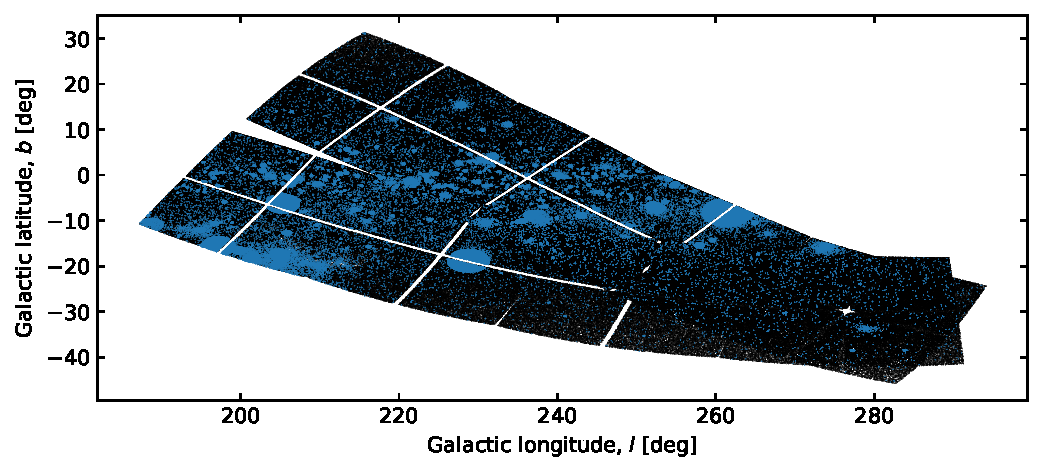
\includegraphics[width=0.9\textwidth]{galacticcoords_cluster_field_star_positions.pdf}
	\end{center}
	\vspace{-0.5cm}
	\caption{
    Positions of light curves from TESS Sectors 6 and 7 in galactic
    coordinates.  Black: $G_{\rm Rp}<13$ field stars.  Blue: $G_{\rm
    Rp}<16$ target stars.  Target stars are mostly near the galactic
    plane. The data for Sectors 6 and 7 cover about one-sixth of the
    galactic plane.
		\label{fig:lcgalactic}
	}
\end{figure*}

%\begin{figure}[!t]
%	\begin{center}
%		\leavevmode
%		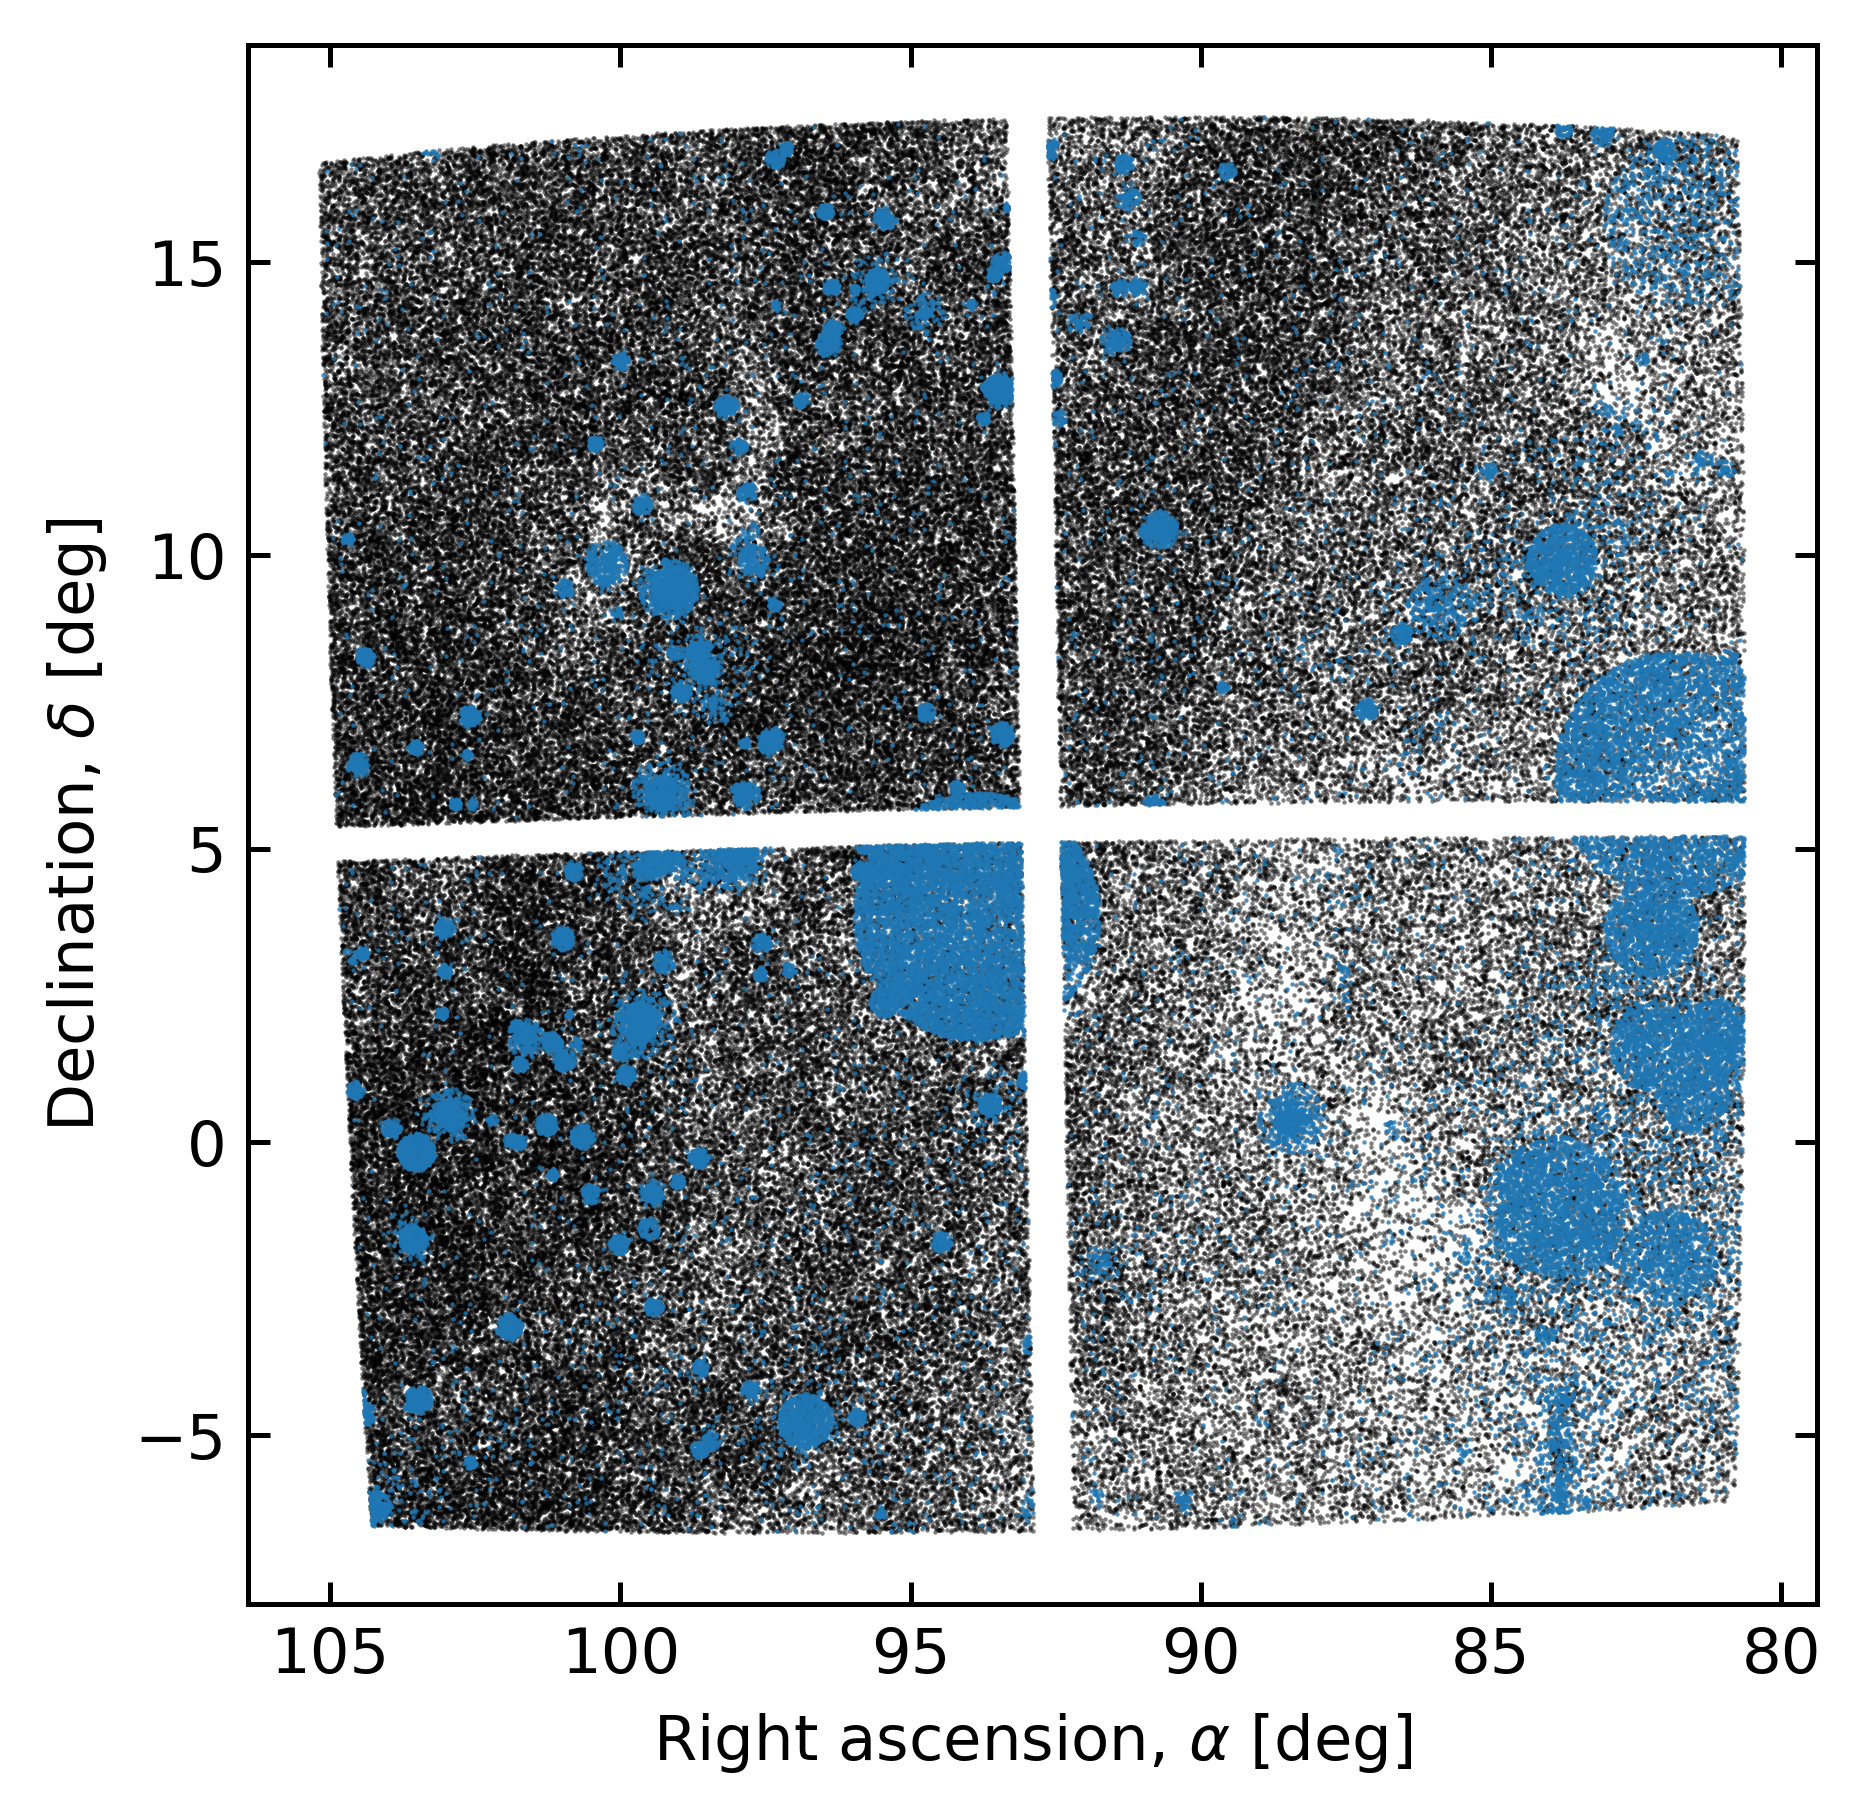
\includegraphics[width=0.47\textwidth]{sector6_cam[1]_ccd[1-2-3-4]cluster_field_star_positions.png}
%	\end{center}
%	\vspace{-0.5cm}
%	\caption{
%		{\bf  Zoom and coordinate transformation
%			of Sector 6, Camera 1 from Figure~\ref{fig:lcgalactic}.}
%		The most populated cluster is XXX, primarily due to candidate
%		members proposed by \citet{dias_proper_2014}.
%		\label{fig:lcradeczoom}
%	}
%\end{figure}


\begin{figure}[!t]
	\begin{center}
		\leavevmode
		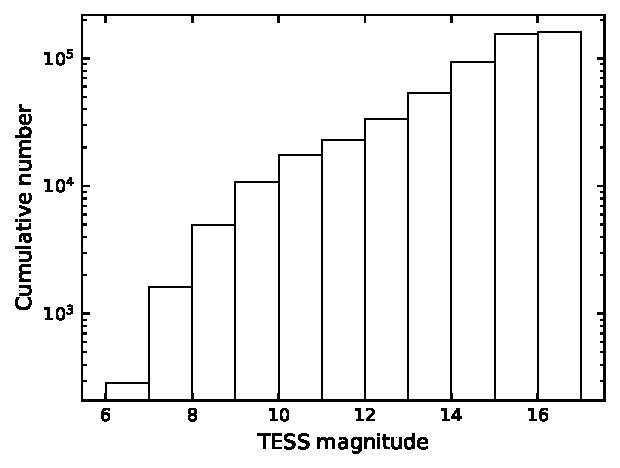
\includegraphics[width=0.45\textwidth]{cdf_T_mag.pdf}
	\end{center}
	\vspace{-0.5cm}
	\caption{
    Cumulative number of CDIPS light curves a function of TESS
    $T$-band magnitude.  Light curves were made for the target stars
    (Figure~\ref{fig:cdips_targets}) that were observed in Sectors 6
    or 7.
		\label{fig:cdf_T_mag}
	}
\end{figure}

\begin{figure}[!ht]
	\gridline{\fig{hrd_scat_all_CDIPS_LCs.pdf}{0.45\textwidth}{}}
	\vspace{-0.8cm}
	\gridline{\fig{hrd_scat_close_subset.pdf}{0.45\textwidth}{}}
	\vspace{-0.8cm}
	\caption{
    {\it Top.} HR diagram of CDIPS stars on silicon in this data
    release.  {\it Bottom.} HR diagram of close CDIPS stars on
    silicon. The wedge separating the pre-MS sample from the MS stars
    was discussed by \citet{zari_3d_2018}, who introduced it in order
    to avoid contamination by photometric binaries.
	}
	\label{fig:hrd}
\end{figure}

\begin{figure}[!t]
	\gridline{\fig{pm_scat_all_CDIPS_LCs.pdf}{0.45\textwidth}{}}
	\vspace{-0.8cm}
	\gridline{\fig{pm_scat_close_subset.pdf}{0.45\textwidth}{}}
	\vspace{-0.8cm}
	\caption{
		{\it Top.} Proper motions of CDIPS stars on silicon in this
		data release.  Many of the stars in the central ``blob'' are possible
		field-contaminants.
		{\it Bottom.} Proper motions of close CDIPS stars
		on silicon.
	}
	\label{fig:propermotions}
\end{figure}

\begin{figure}[!t]
	\begin{center}
		\leavevmode
		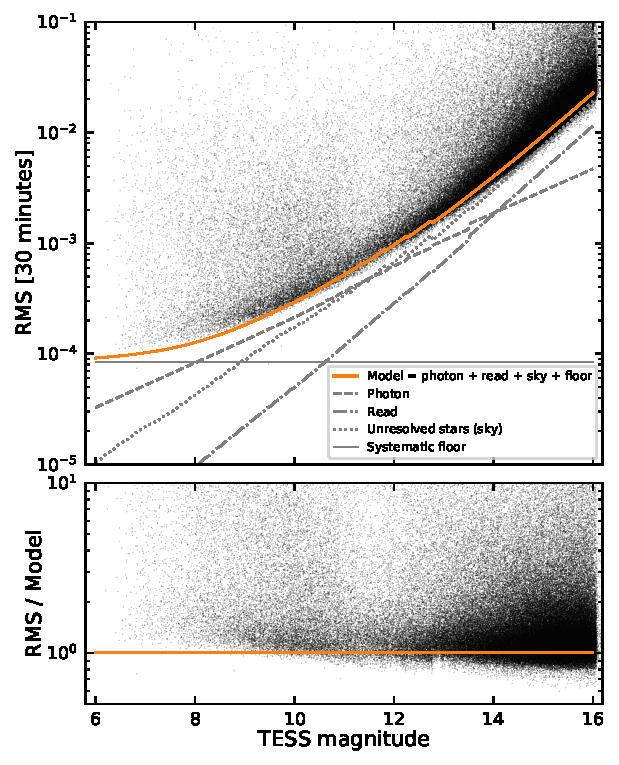
\includegraphics[width=0.47\textwidth]{rms_vs_mag.pdf}
	\end{center}
	\vspace{-0.5cm}
	\caption{
    Standard deviation of TFA-detrended CDIPS light curves as a
    function of catalog TESS-band magnitude.  Black points correspond
    to the minimum RMS across the available three aperture sizes.  The
    model (orange and gray lines) assumes aperture sizes reported by
    \citet{Sullivan_et_al_2015}, and the effective area from
    \citet{vanderspek_2018}.  The noise from unresolved background
    stars (dotted gray line) is a function of galactic latitude, and
    dominates over zodiacal light for faint stars near the galactic
    plane; the line shown assumes a sight-line towards the center of
    Sector 6, Camera 1 (further details are in
    \S~\ref{subsubsec:rmsvsmag}).
		\label{fig:rms_vs_mag}
	}
\end{figure}

\begin{figure}[!t]
	\begin{center}
		\leavevmode
		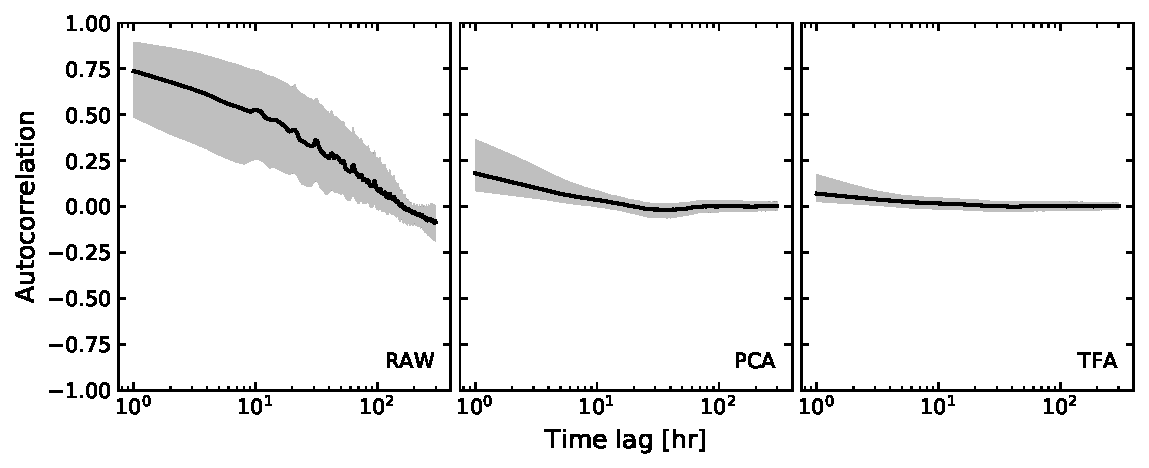
\includegraphics[width=0.47\textwidth]{avg_acf.pdf}
	\end{center}
	\vspace{-0.5cm}
  \caption{
    Average autocorrelations of $10^4$ randomly selected light curves
    from each sector.  The medians at time lags spaced by one hour are
    shown for raw light curves (column name \texttt{IRM}) in gray, and
    for TFA-detrended light curves in black.  The gray bands display
    the 25$^{\rm th}$ to 75$^{\rm th}$ percentile range for each type
    of light curve.
  \label{fig:avg_acf}
	}
\end{figure}


\subsection{Light Curve Statistics}
\label{subsec:lcstatistics}

\subsubsection{Stellar properties}

The on-sky locations of the light curves from Sectors 6 and 7 are
shown in Figure~\ref{fig:lcgalactic}.  Black stars are the field stars
for which we performed photometry, and of which a subset were used as
template stars during TFA.  The blue stars are the \numberlcs stars
with light curves available from \stscilink.  Most of the target stars
are quite close to the galactic plane.  Gaps between CCD chips are
also visible.  The highly clumped nature of the target stars is also
apparent.

%A zoom-in of Figure~\ref{fig:lcgalactic} is shown in Figure~\ref{fig:lcradeczoom}
%for the Camera 1, Sector 6 field. The effects of galactic-latitude
%dependent extinction are visible through the decreasing density of black
%points towards the right of the image.

Figure~\ref{fig:cdf_T_mag} shows the cumulative distribution of TESS
$T$-band magnitudes for the target stars.  Though most of the targets
are faint, $\approx3\times10^4$ are brighter than $T=13$. These
targets are more promising for any detailed follow-up observtions.

An HR diagram for the entire sample of CDIPS stars on silicon is shown
in Figure~\ref{fig:hrd} (top).  The sub-sample of stars with measured
positive parallaxes and naive distances less than $1\,{\rm kpc}$ is
also shown (bottom).  About one-third of the stars are in this latter
sample.  The close stars are predominantly on the main-sequence, or
the pre-main-sequence.  A relatively large fraction of these come from
\citet{zari_3d_2018}, and are either on the PMS or upper
main-sequence.  The latter set of OBA dwarf stars, while ``younger''
than the typical field dwarf, are likely the least interesting subset
of our target sample from the perspective of age analyses.  In the
entire sample (Figure~\ref{fig:hrd} top), a much larger fraction of
stars are sub-giants, red giants, and helium-burning red-clump stars.
We failed to obtain light curves for roughly $5\%$ of the stars on
silicon, primarily due to our masking of saturated stars and their
nearby pixels.

Finally, Figure~\ref{fig:propermotions} shows the proper motions of
the entire and close samples of stars on silicon.  Each clump
signifies a different star cluster. The largest overdensity in the top
figure is composed mainly of field star contaminants. It has two
subcomponents, due to the two different directions in the Galaxy being
observed in Sectors 6 and 7.



\subsubsection{Cluster membership provenance}

\paragraph{Sector 6}
In Sector 6, \sVInumberlcs light curves of candidate cluster stars
were made. The provenance of the claimed cluster origin of these
sources is \citet{dias_proper_2014} for 59\% of the sources;
\citet{zari_3d_2018} for 16\% of sources from their upper
main-sequence table and 1\% of sources from their PMS table;
\citet{Kharchenko_et_al_2013} for 8\% of sources,
\citet{cantat-gaudin_gaia_2018} for 6\% of sources, and more than two
catalogs for the remaining 10\% of sources.

The clusters with the largest claimed numbers of sources are the
Platais~6, Platais~5, and Mamajek~3 moving groups, all from
\citet{dias_proper_2014}, composing about 7000, 7000, and 3500 sources
respectively. These membership claims should be regarded with some
skepticism on a source-by-source basis.  For Platais~6,
\citet{Kharchenko_et_al_2013} claimed only about 400 probable members
(1$\sigma$) to exist within the angular radius of the cluster.
Mamajek~3 (= 32$\,$Ori) has only about 50 confirmed members
\citep{bell_32ori_2017}.

We remind the reader that our goal in creating our target catalog was
completeness, rather than fidelity. The \citet{dias_proper_2014} stars
in particular were included if they were listed with membership
probability exceeding 50\%.  To create cleaner sub-samples, we advise
use of the \texttt{CDEXTCAT} header keyword, which can be used to
merge against the original source catalog to obtain the membership
probabilities claimed by the original catalog.

\paragraph{Sector 7}
In Sector 7, \sVIInumberlcs light curves of candidate cluster stars
were made. The provenance of the claimed cluster origin of these
sources is  ... LGBTODO

The clusters with the largest claimed numbers of sources are ...
LGBTODO

\subsubsection{Light curve noise properties}
\label{subsubsec:rmsvsmag}

\paragraph{Observed RMS vs magnitude.}
The standard deviation of the TFA-detrended light curves is plotted as
a function of the catalog $T$-band magnitude for CDIPS light curves in
Figure~\ref{fig:rms_vs_mag}.
For the $y$-axis of this plot, we have taken
\begin{equation}
  {\rm RMS} = \left[
    \frac{1}{N-M-1}
    \sum_{i=1}^{N} (f_i - \bar{f})^2
  \right]^{1/2},
\end{equation}
where $f_i$ is the value of the flux at the $i^{\rm th}$ point in the
time-series, $\bar{f}$ is the mean flux, $N$ is the
number of points in the time-series, and $M$ is the number
of template light curves used during TFA detrending.
The correction in the denominator penalizes the natural degree of
overfitting inherent to the TFA algorithm.

The observed RMS (black points) follows the usual shape, with photon
noise dominating from $T=9$ to $T=12$, beyond which the onset of the
``sky'' background changes the overall slope of the curve to be more
steep.  For the brightest stars ($T\lesssim 9$), a ``systematic
floor'' was part of the mission's error budget
\citep{ricker_transiting_2015}, but has not been observed in early
reports of the photometric performance of various aperture photometry
pipelines ({\it e.g.,} the SPOC pipeline \citealt{jenkins_spoc_2010},
the MIT-QLP \citealt{huang_tess_2018}, and \texttt{eleanor}
\citealt{feinstein_eleanor_2019}).  The fact that our light curves for
the brightest stars are above this purported ``floor'', rather than
below it, suggests that our image subtraction techniques could be
introducing some small degree of noise to the light curves of the
brightest stars.  It is also true however that our largest aperture
contains only about 16 pixels, which is sub-optimal for stars brighter
than $T\approx9$ \citep[see][Figure~14]{Sullivan_et_al_2015}.  Since
the brightest stars are not the focus of the present work, we leave
this issue unaddressed for the time being.

Importantly, the faint stars do not noticeably exhibit
the typical effects of crowding at the faint end 
\citep[{\it e.g.},][Figure~5]{feinstein_eleanor_2019}.
In aperture photometry pipelines, stars in very crowded regions typically 
have their flux overestimated relative to the actual number of photons
that fall on silicon.
This leads to systematic underestimates of the uncertainty in the relative 
fluxes, as well as ``flux contamination'' (the reduction in amplitude of say, 
transit signals, due to diluting flux from neighbor stars).
Our method to work around this problem -- using the catalog magnitudes to 
predict the reference flux values, and measuring deviations from these 
reference fluxes on the subtracted images -- seems to be performing well.


\paragraph{Expected RMS vs magnitude.}

The noise model shown in Figure~\ref{fig:rms_vs_mag} is quite similar
to that of \citet{Sullivan_et_al_2015}, save for two changes.
The first change is that the effective area of the telescope is
updated to be $86.6\,{\rm cm}^2$, per the measurements by
\citet{vanderspek_2018}.

The second change is that we have explicitly included the
estimated noise contribution from unresolved faint stars.  The
brightness of the diffuse sky is dominated by different sources at
different wavelengths.  For instance, the CMB is most important in
the microwave, and thermal radiation from dust grains in the solar
system (zodiacal light) is dominant in the far infra-red
\citep{leinert_1997_1998}.  In the TESS-band, both zodiacal light and
faint stars can play a role, depending on the line of sight under
consideration. The zodiacal light is brightest near the ecliptic
plane, and the faint star background is brightest near the galactic
plane (and towards the galactic center).  
When performing pre-launch noise estimates,
\citet{winn_background_2013}
estimated the photon-counts from each component.
His zodiacal light model was presented by \citet{Sullivan_et_al_2015},
but the faint star component was not emphasized since the Sullivan
simulations were performed away from the galactic plane.

The diffuse sky model we have used for Figure~\ref{fig:rms_vs_mag} is
adopted explicitly because most of our target stars are near the
galactic plane.
Stars are judged to be ``unresolved'' and part of the background if
their surface density exceeds the angular resolution of the telescope.
TESS has an angular resolution of $\Delta \theta \sim 1'$, set by a
combination of the pixel size as well as the typical stellar FWHM.
Sources with sky surface density exceeding $\Delta \theta^{-2}$
therefore contribute to the background.

The relevant quantity needed to calculate the integrated 
photon counts from faint sources
is  $N(<m,l,b)$ --- the number of stars per square arcsecond
brighter than magnitude $m$, along a line of sight with galactic
longitude and latitude $(l,b)$.
To calculate this surface density, \citet{winn_background_2013}
queried the Besan\c con model
\citep{robin_synthetic_2003}  along a grid of galactic sight-lines,
and then converted to $I$-band surface brightnesses.
Fitting a smooth function to the results, \citet{winn_background_2013}
found
\begin{equation}
I\ {\rm mag\ arcsec}^{-2} =
    a_0 + a_1 \left(\frac{|b|}{40^\circ}\right)
    + a_2 \left(\frac{|l|}{180^\circ}\right)^{a_3},
\end{equation}
where the galactic longitude $l$ is measured from $-180^\circ$ to
$180^\circ$, and the empirical coefficients were found to be $a_0 =
18.9733$, $a_1=8.833$, $a_2=4.007$, and $a_3=0.805$.  This fit was
cautioned to be {\it very approximate}.  It is sensitive to the
threshold used to select ``unresolved'' stars, and likely no more
accurate than 0.5 mag on average.  In regions with exceptionally high
extinction ({\it e.g.}, star forming regions) it is expected to
systematic underestimate the background brightness by an even larger
degree.
Nonetheless, this model for the diffuse sky background seems
to agree reasonably well with the observed trend of standard deviation
versus stellar magnitude.


\paragraph{ACF statistics}

Beyond the white noise properties of the light curves, the red noise
properties are also important. 
In Figure~\ref{fig:avg_acf} we show the average autocorrelation of the
raw and TFA-filtered light curves.
The raw light curves have substantial systematic red noise; 
their average autocorrelation, evaluated at various time lags, is
positive.
The TFA-filtered light curves are much closer to gaussian~--~the
average autocorrelation between any two points in these light curves
is close to zero.
However, the average TFA-filtered light curve is not {\it exactly}
gaussian.
At time lags of a few hours or less, there is some excess power.
This suggests that additional detrending may be
necessary to maximize the effectiveness of planet searches (or the discovery of
any other signals via matched-filter techniques).


\subsection{A Few Objects of Interest}
\label{subsec:identifying_variability}

\begin{figure}[!t]
	\gridline{\fig{tls_sde_vs_period_scatter.pdf}{0.45\textwidth}{}}
	\vspace{-0.8cm}
	\caption{
    Transiting planet search periodogram summary.
    Each point represents the TLS periodogram peak signal detection
    efficiency (SDE) and corresponding period from one light curve.
    Significance thresholds (orange lines) are empirically defined for
    the transiting planet search described in
    \S~\ref{subsec:identifying_variability}.  
    {\it Top.} Sector 6.  {\it Bottom.} Sector 7.
	}
	\label{fig:tlsresults}
\end{figure}

We will discuss our search for transiting planets in an upcoming
report.  To identify an initial set of transiting planets, strong
stellar rotators, and eclipsing binaries, we performed a few steps of
post-processing on the light curves.  This processing was done
independently of the data release, since it was quite specific to our
own scientific interests.  The code used to do this additional
processing is also available
online\footnote{\url{github.com/lgbouma/cdips}, commit
\texttt{348eea7}.}.

%FIXME
%FIXME
%FIXME
%FIXME


%%%%%%%%%%%%%%%%%%%%%%%%%%%%%%%%%%%%%%%%%%
\section{Conclusion}
\label{sec:conclusion}

%FIXME: paraphrase / improve all the below
In this study, we first collected an all-sky sample of about one million
candidate young stars brighter than $G_{\rm Rp}$ of 16.
82\% of the target star sample resides in a ``cluster'', a generic
term we adopted for open clusters, stellar associations, and moving
groups.
The remaining stars have photometric or astrometric indications of
their youth, and either reside on the pre-main-sequence or upper
main sequence.

We then reduced TESS full frame images taken over the course of about
two months (Sectors 6 and 7; the first fields very close to the galactic
plane).
We performed difference imaging in order to minimize the complications
of the crowded background.
Using forced aperture photometry, we made light curves for all stars
brighter than $G_{\rm Rp}$ of 13, and went three magnitudes deeper for
our target star sample.
This yielded \numberlcs light curves of candidate young stars across
\numberclusters distinct clusters.

The light curves seem to be limited in precision by photon noise at
the bright end, and by unresolved background stars at the faint end.
Though the raw light curves show significant red noise, decorrelating
against a set of template stars led to an ensemble of light curves
with very nearly gaussian noise properties.

An initial search for objects that were photometrically variable
returned pulsating stars, eclipsing binaries, and planet candidates.
A detailed planet search is the subject of ongoing work.
An of the stars in the sample must be understood to be {\it candidate}
cluster stars, and the possibility of photometric blends 
is important to rule out in subsequent vetting efforts of any variable
object.

As a brief exploration of the photometric variability in the dataset,
we looked at the age-evolution of extremely high-SNR variability,
which seems to show some evolution in the space of LS peak-period
versus color (Figure~\ref{fig:ls_peak_vs_time}), but interpreting this
result will require a more careful exploration.  In searching for
transiting planets, we found many eclipsing binaries, as well as
stellar rotation and pulsation signals.

Those who wish to explore the
time-evolution in these and any other systems are invited to explore
the data at \stscilink.





\acknowledgements
L.G.B.\ gladly acknowledges helpful discussions with
C Huang, M Soares-Furtado, ...
..., and is
grateful to the people who have turned TESS from an idea into reality.
%
J.N.W.\ thanks ...
%
This paper includes data collected by the TESS mission, which are
publicly available from the Mikulski Archive for Space Telescopes
(MAST).
%
Funding for the TESS mission is provided by NASA's Science Mission
directorate.
%
This research has made use of the NASA Exoplanet Archive, which is
operated by the California Institute of Technology, under contract
with the National Aeronautics and Space Administration under the
Exoplanet Exploration Program.
%
This work made use of NASA's Astrophysics Data System Bibliographic
Services.
%
This research has made use of the VizieR catalogue access tool, CDS,
Strasbourg, France. The original description of the VizieR service was
published in A\&AS 143, 23.
%
This work has made use of data from the European Space Agency (ESA)
mission {\it Gaia} (\url{https://www.cosmos.esa.int/gaia}), processed
by the {\it Gaia} Data Processing and Analysis Consortium (DPAC,
\url{https://www.cosmos.esa.int/web/gaia/dpac/consortium}). Funding
for the DPAC has been provided by national institutions, in particular
the institutions participating in the {\it Gaia} Multilateral
Agreement.
%
The Digitized Sky Surveys were produced at the Space Telescope Science
Institute under U.S. Government grant NAG W-2166. The images of these
surveys are based on photographic data obtained using the Oschin
Schmidt Telescope on Palomar Mountain and the UK Schmidt Telescope.
The plates were processed into the present compressed digital form
with the permission of these institutions.
%
\newline
%
\facility{
	2MASS \citep{skrutskie_tmass_2006},
	Gaia \citep{gaia_collaboration_gaia_2016,gaia_collaboration_gaia_2018},
	TESS \citep{ricker_transiting_2015},
	UCAC4 \citep{zacharias_fourth_2013}
    %DSS (CITE)    
}
%
\software{
  \texttt{astrobase} \citep{bhatti_astrobase_2018},
  \texttt{astropy} \citep{the_astropy_collaboration_astropy_2018},
  \texttt{astroquery} \citep{astroquery_2018},
  %\texttt{astroquery.gaia} CITE,
  %\texttt{astroquery.simbad} CITE,
  %\texttt{astroquery.mast} CITE,
  %\texttt{astroquery.nasaexopanetarchive} CITE,
  \texttt{BATMAN} \citep{kreidberg_batman_2015},
  \texttt{corner} \citep{corner_2016},
  \texttt{emcee} \citep{foreman-mackey_emcee_2013},
  \texttt{fitsh} \citep{Pal_2012},
  \texttt{IPython} \citep{perez_2007},
  \texttt{matplotlib} \citep{hunter_matplotlib_2007}, 
  \texttt{numpy} \citep{walt_numpy_2011}, 
  \texttt{pandas} \citep{mckinney-proc-scipy-2010},
  \texttt{pyGAM} \citep{serven_pygam_2018_1476122}
  \texttt{psycopg2} (\url{initd.org/psycopg})
  \texttt{scipy} \citep{jones_scipy_2001},
  \texttt{scikit-learn} \citep{sklearn_2011},
  \texttt{TagSpaces} (\url{tagspaces.org}),
  \texttt{tesscut} \citep{brasseur_astrocut_2019},
  \texttt{VARTOOLS} \citep{Hartman_Bakos_2016}
  \texttt{wotan} \citep{hippke_wotan_2019},
}

\clearpage
\newpage

\bibliographystyle{yahapj}                            
\bibliography{bibliography} 

\appendix
\section{Time system \& barycentric correction}
\label{appendix:time}

The time-stamps included with the calibrated TESS Full Frame Images
produced by SPOC include a barycenteric correction at
a single reference pixel given at the middle of every frame.
The barycentric correction is at maximum 16 minutes, corresponding to
points on the sky separated by 180 degrees.
The angular distance from a TESS camera's center of field to the corners
is $\approx$17 degrees, so naively one might incur at worst an error of
$\approx$90 seconds on the time-stamps due to using a barycentric
correction in a direction that is slightly wrong.
Perhaps due to the lead author's obsession with getting time-stamps correct 
\citep{bouma_wasp-4b_2019},
we perform our own barycentric correction using the appropriate
sky coordinates for each light curve.
We advise use of our \texttt{TMID\_BJD} column, which gives the
mid-time of each exposure in the BJD$_{\rm TDB}$ time system, which
is the defacto standard in exoplanet and stellar
astronomy~\citep{eastman_achieving_2010}.

\section{Assigning unique names to each cluster}
\label{appendix:uniquenames}

In assigning a single unique cluster name to each star, we matched
against the \citet{Kharchenko_et_al_2013} name whenever possible,
since this was the largest available catalog, and it also included
homogeneous age determinations for many of the clusters.
To find the matching name, in order of precedence we
\begin{enumerate}
  \item Checked for direct string matches from
    \citet{Kharchenko_et_al_2013} clusters with determined parameters;
  \item Checked whether the SIMBAD online name resolving service \citep{wenger_simbad_2000} had
    any direct string matches against \citet{Kharchenko_et_al_2013}
    clusters with determined parameters;
  \item Checked for string matches in the full
    \citet{Kharchenko_et_al_2013} index (including clusters without
    determined parameters);
  \item Searched for spatial matches between each star and cluster
    centers from \citet{Kharchenko_et_al_2013} within 10 arcminutes.
    In cases with multiple cluster matches, we ignored candidate
    matches to avoid assigning incorrect names;
  \item Checked the WEBDA double name
    list\footnote{\url{https://webda.physics.muni.cz/double_names.html}},
    and repeated Steps 1-4 with any matches.
\end{enumerate}

A few edge-cases, including for instance sub-clusters  larger
star-forming complexes like in Sco-Cen or Collinder~33, were 
manually resolved to the extent feasible (\citealt{rizzuto_multidimensional_2011}
and \citealt{saurin_isolating_2015} give
detailed pictures of the complex morphologies that frequently arise in
young star-forming regions).

The procedure described above failed to yield matches for a few of the
infrared clusters identified by \citet{majaess_discovering_2013} and
included in the \citet{dias_proper_2014} catalog.
For these cases, we used the name given by \citet{dias_proper_2014}.
The larger set of ``FSR'' infrared clusters from
\citet{froebrich_FSR_2007} was incorporated to
\citet{Kharchenko_et_al_2013}, and so did not present any
complications.

The Hyades and a number of other nearby moving groups were also
missed, since they were not in the \citet{Kharchenko_et_al_2013}
catalog.  For moving groups not identified in
\citet{Kharchenko_et_al_2013}, we adopted the constellation-based
naming convention from \citet{gagne_banyan_XI_2018}.  

Finally, the procedure enumerated above did not yield matches for
recently discovered clusters, such as the ``RSG'' clusters found by
\citet{roser_nine_RSG_2016} and the ``Gulliver'' clusters from
\citet{cantat-gaudin_gaia_2018}.  In these cases, we used the names
given by the original authors.

\end{document}

